%!TEX root = ../thesis.tex
% ******************************* Thesis Appendix B ********************************

\chapter{Additional information to Chapter 4} \label{appendix:CTsub}
This Appendix contains supplementary figures for Chapter~\ref{chap:CT_bio}.


\section{Supplementary Figures}
\label{sectionB1.1}

\begin{figure}[ht!] 
\centering    
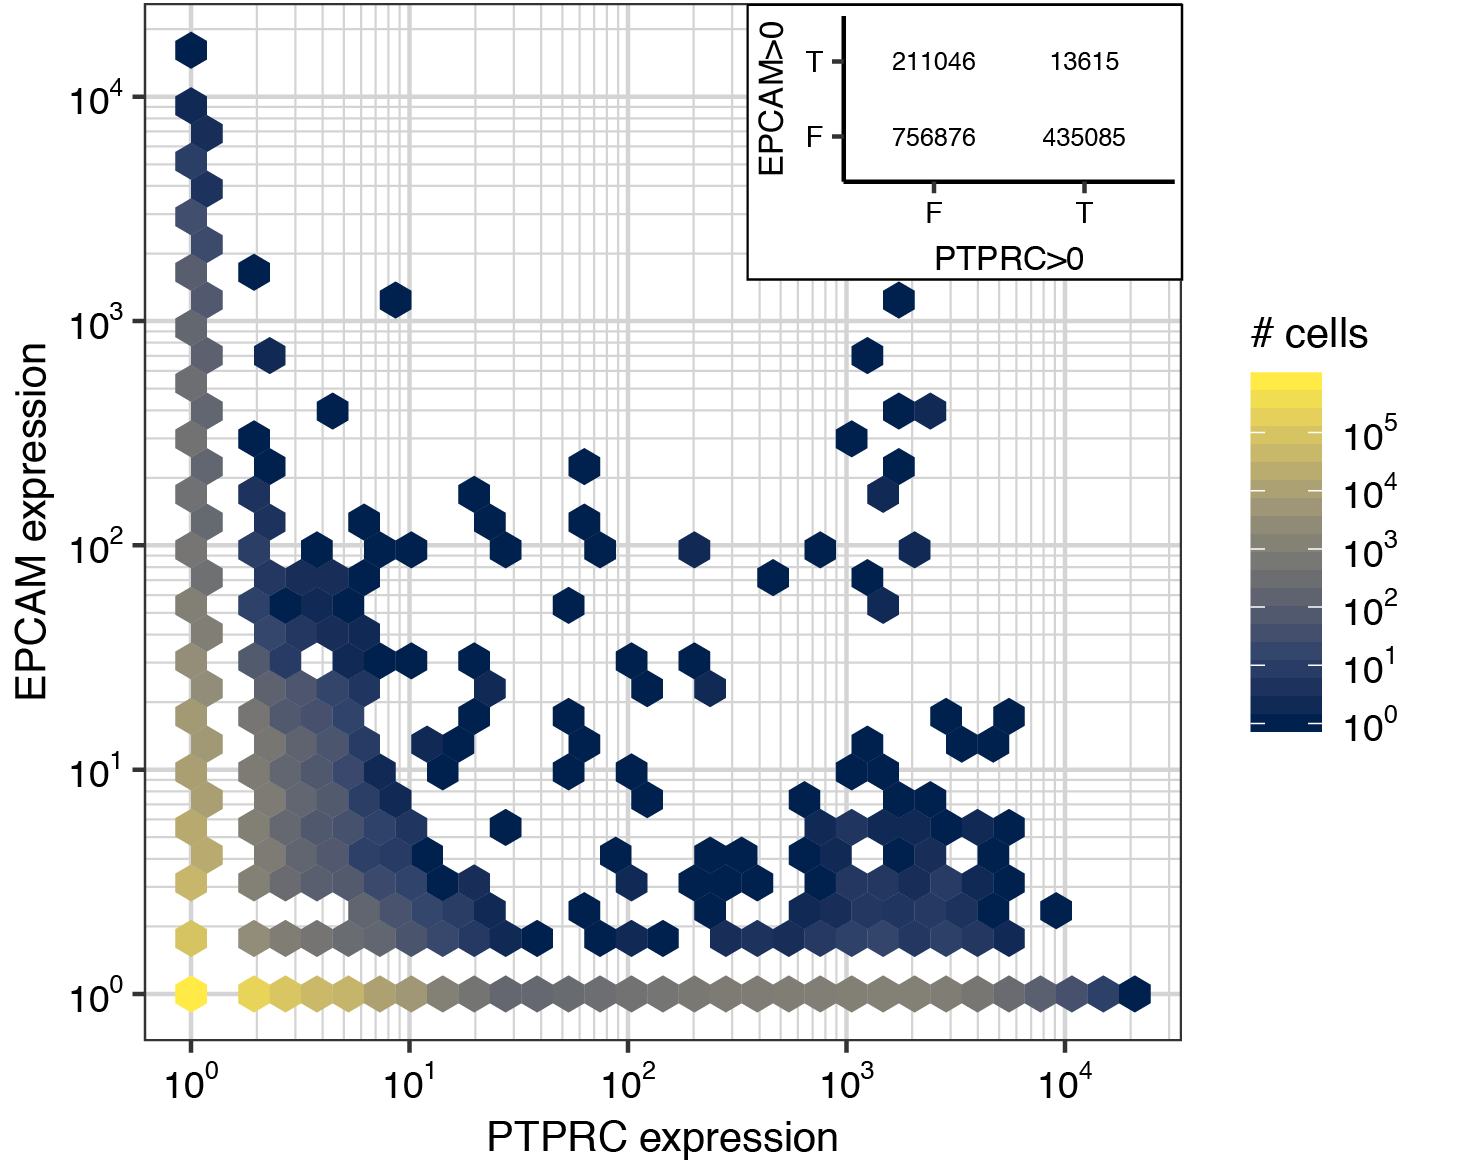
\includegraphics[scale=0.81]{Appendix2/Figs/PTPRC_EPCAM_human.png} % change word in curlies to change figure
\caption[Expression of \textit{PTPRC} and \textit{EPCAM} in human data collection]{\textbf{Expression of \textit{PTPRC} and \textit{EPCAM} in human data collection (Related to Figure~\ref{fig:chap4_cha})}\newline2D-binned plot of single-cell expression of \textit{PTPRC} (encoding for the CD45 receptor, an immune cell marker), and \textit{EPCAM} (an epithelial cell marker). Inset table (top right) shows the number of cell expressing (T) or not (F) each of the genes. Cells expressing both genes are likely doublets or affected by ambient RNA in droplet-based experiments.}
\label{fig:appB_ptprc}
\end{figure}


\begin{figure}[ht!] 
\centering    
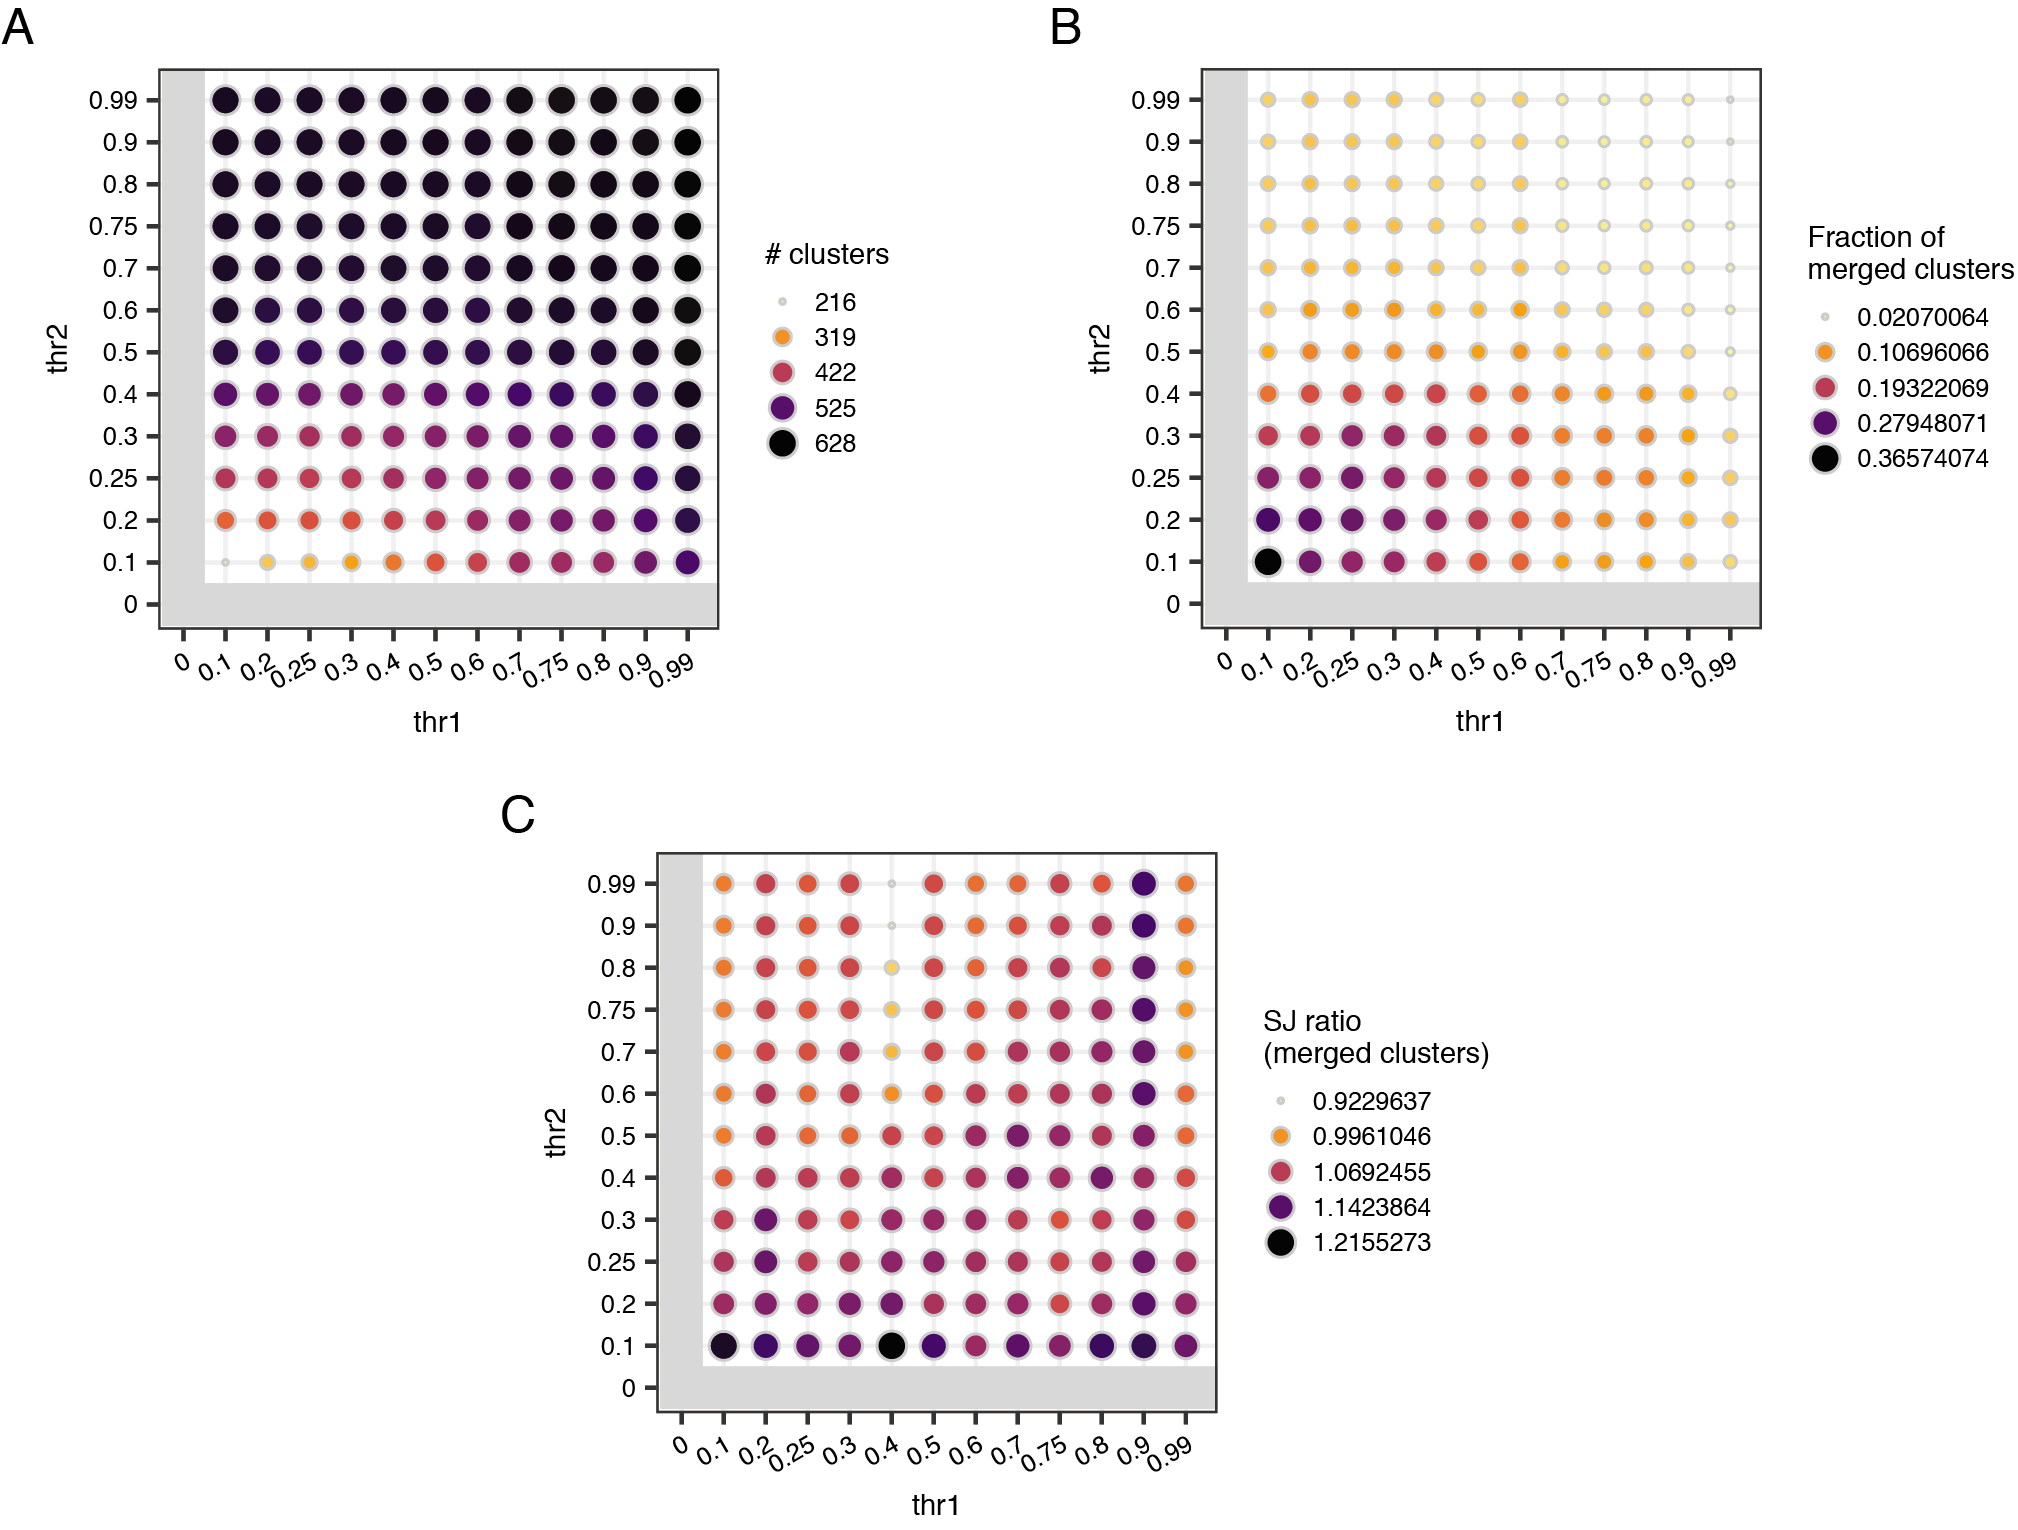
\includegraphics[width=1.0\textwidth]{Appendix2/Figs/chap4_grids.png} % change word in curlies to change figure
\caption[\textit{CellTypist} parameters grids with other statistics]{\textbf{\textit{CellTypist} parameters grids with other statistics (Related to Figure~\ref{fig:chap4_HA})}\newline Parameter grids for \textit{CellTypist} showing variation in \textbf{(A)} total number of clusters; \textbf{(B)} fraction of merged clusters; \textbf{(C)} SJ ratio calculated only for merged clusters.}
\label{fig:appB_grids}
\end{figure}


\begin{figure}[ht!] 
\centering    
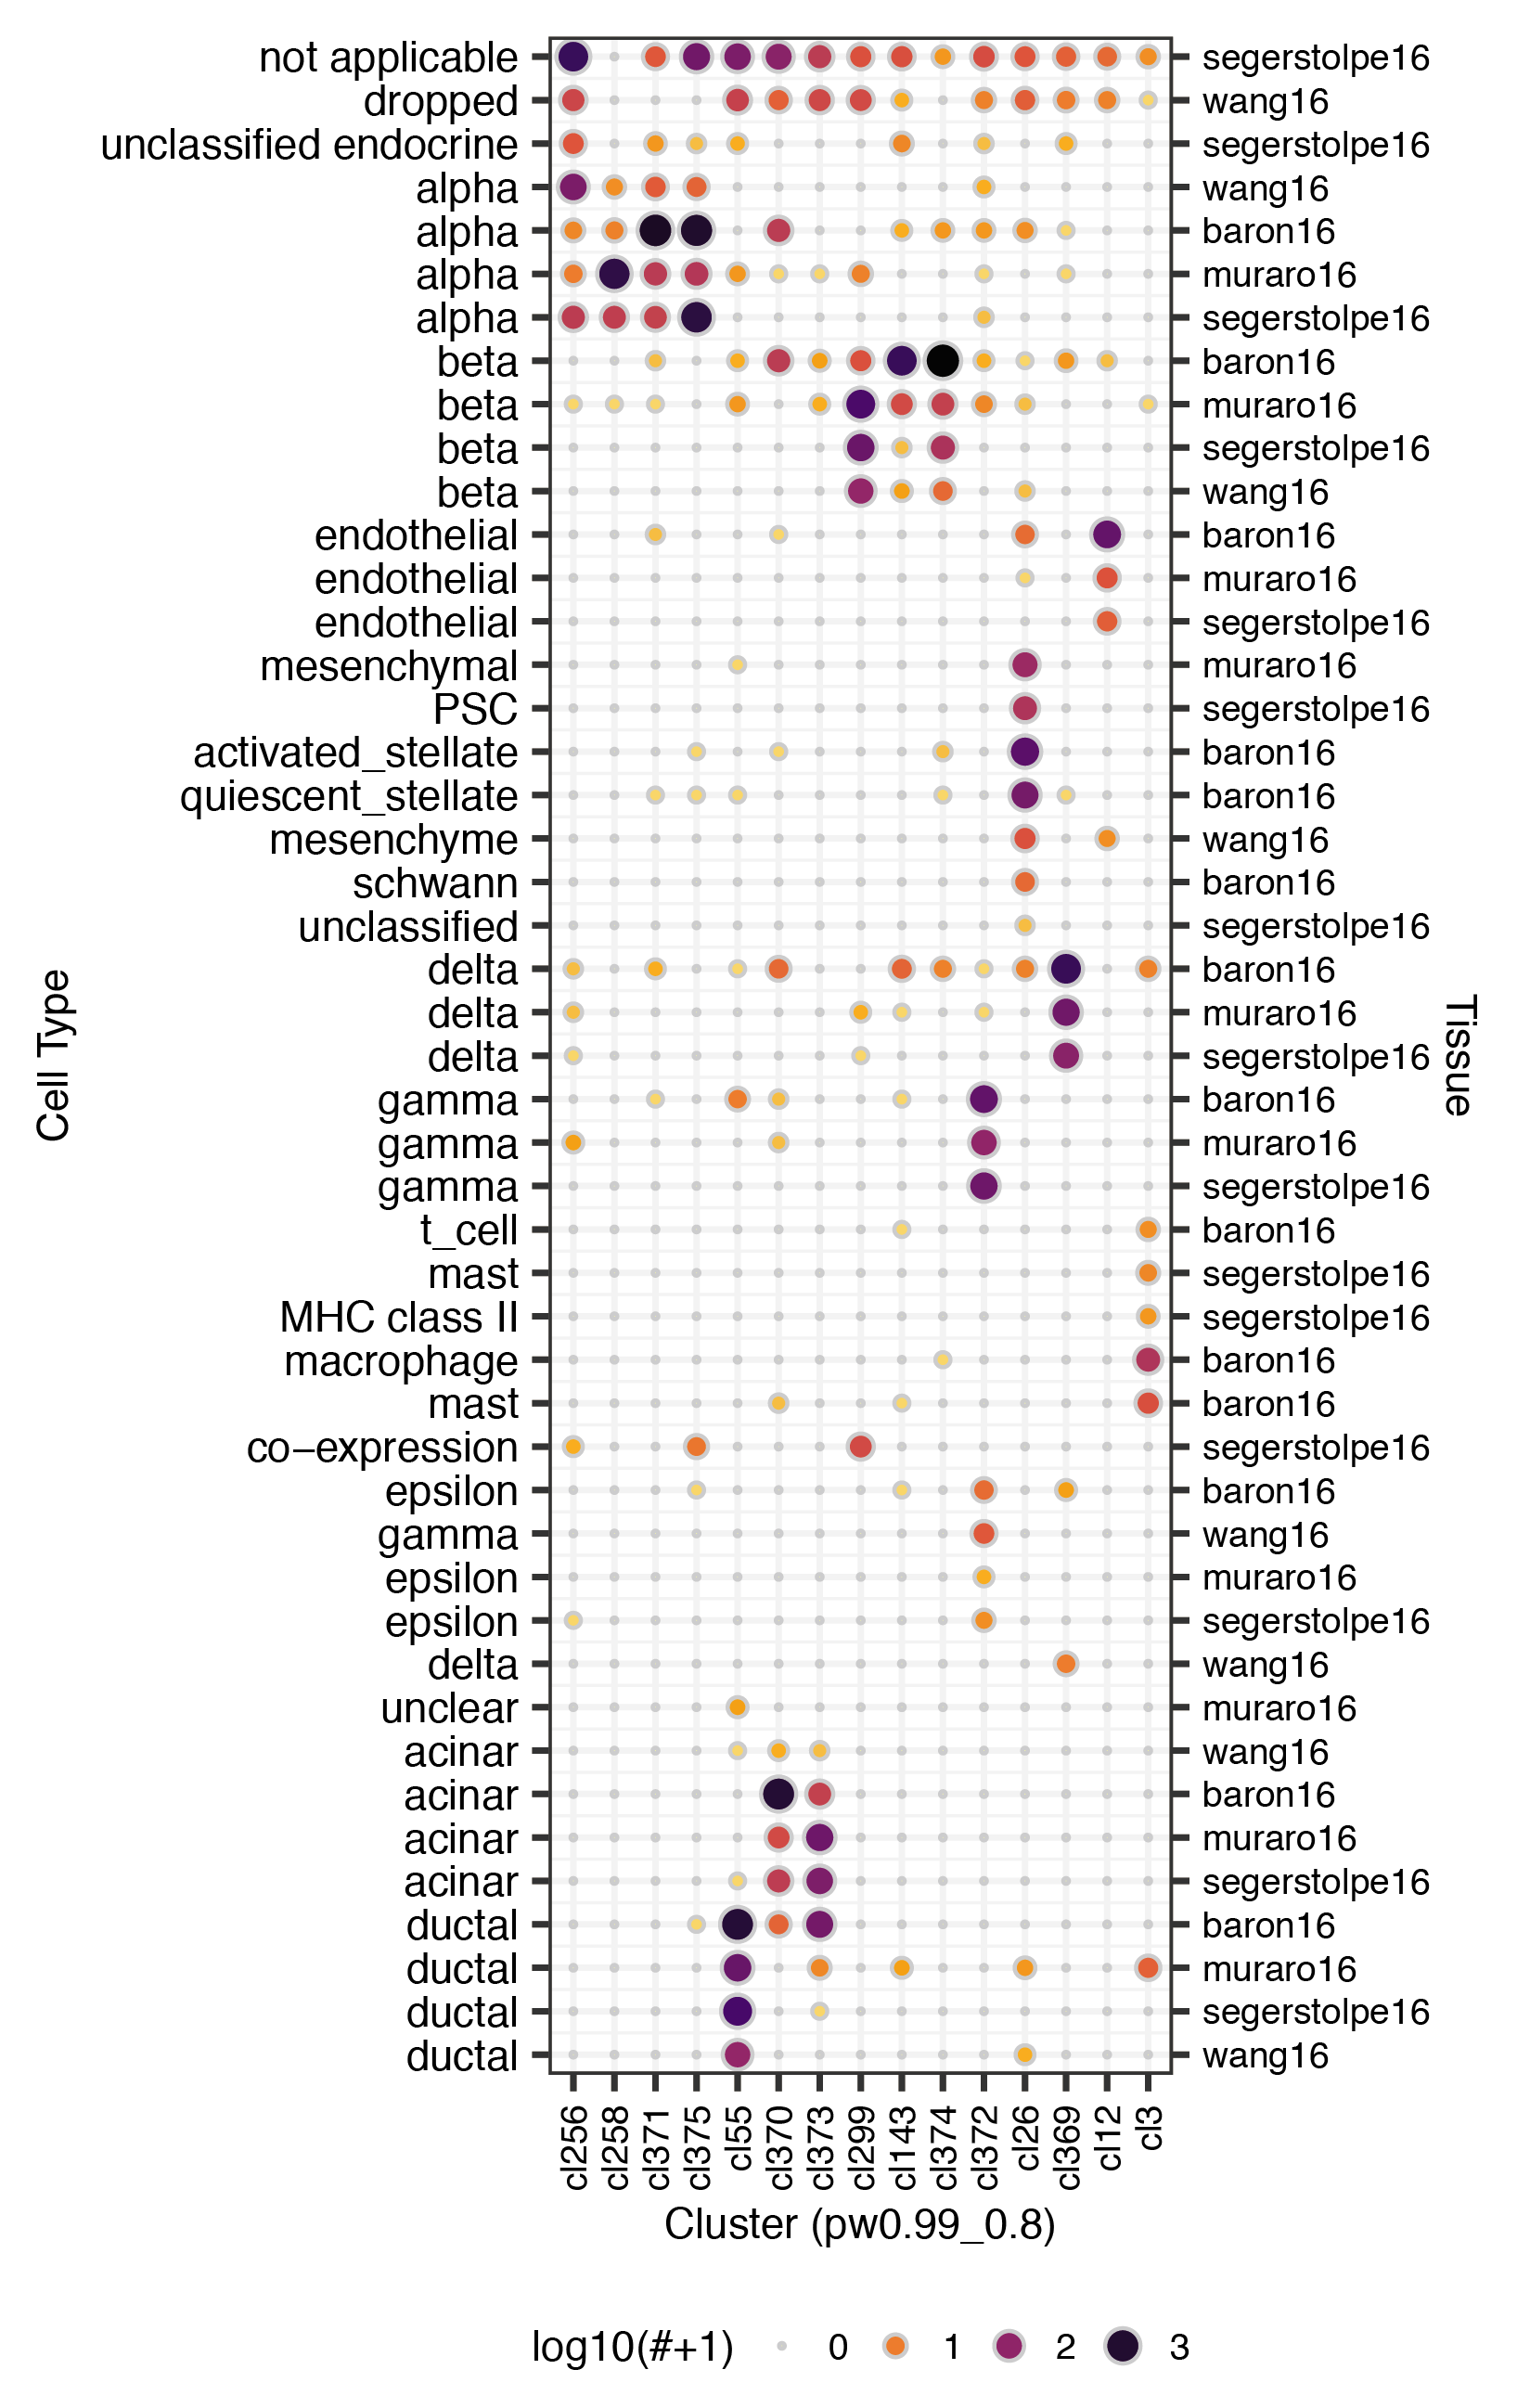
\includegraphics[scale=0.85]{Appendix2/Figs/appB_ctclpancreas.png} % change word in curlies to change figure
\caption[Grouping of annotated cell types and datasets in human pancreas data]{\textbf{Grouping of annotated cell types and datasets in human pancreas data (Related to Figure~\ref{fig:chap4_HA})}\newline Number of cells of each cluster coming from a specific dataset (right y-axis), with a particular cell type annotation (left y-axis). Pancreas was used for this example due to the consistent cell type annotations used across datasets. \textit{CellTypist} parameters: thr1 = 0.99; thr2 = 0.8.}
\label{fig:appB_panc}
\end{figure}


\begin{figure}[ht!] 
\centering    
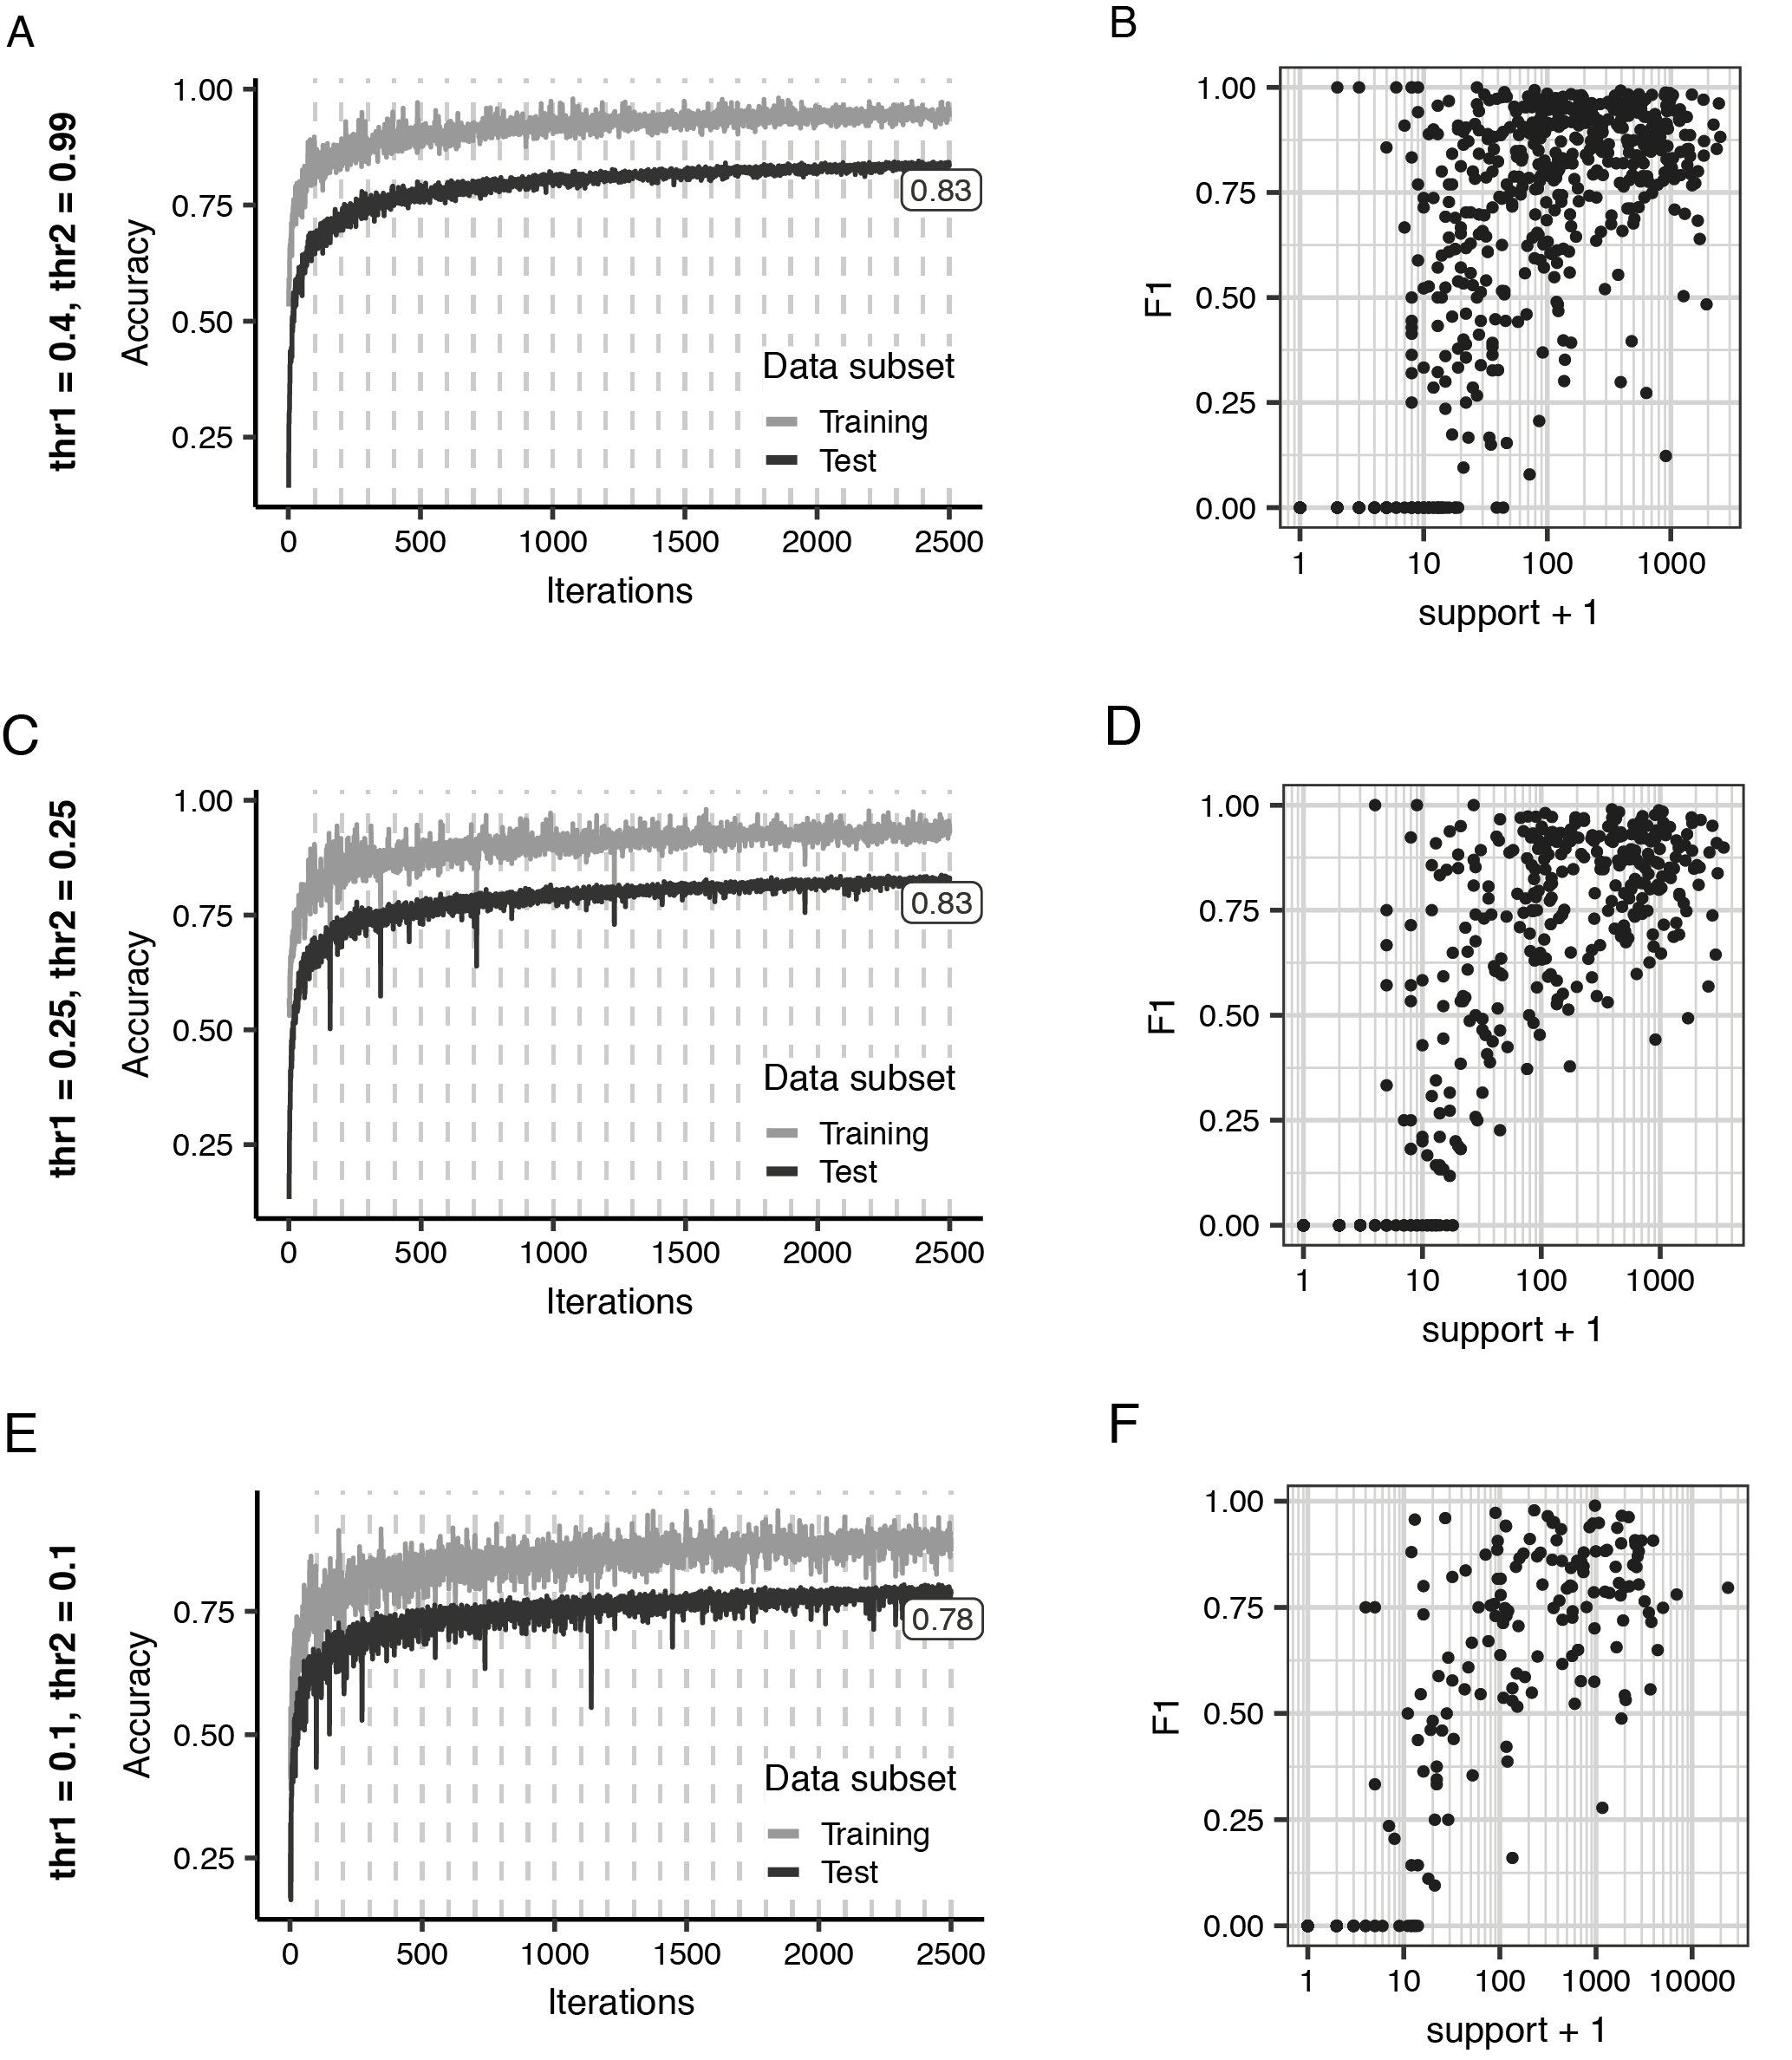
\includegraphics[width=1.0\textwidth]{Appendix2/Figs/appB_modelstuff.png} % change word in curlies to change figure
\caption[Training statistics for other \textit{CellTypist} models]{\textbf{Training statistics for other \textit{CellTypist} models (Related to Figure~\ref{fig:chap4_HA})}\newline For each model trained (thr1 = 0.4 and thr2 = 0.99 - top; thr1 = 0.25 and thr2 = 0.25 - middle; thr1 = 0.1 and thr2 = 0.1 - bottom): \textbf{(A, C, E)} accuracy during model fitting for training and held-out test data; \textbf{(B, D, F)} F1-score for each cluster label (black dots) as a function of class size (in log10 scale).}
\label{fig:appB_moremodels}
\end{figure}


\begin{figure}[ht!] 
\centering    
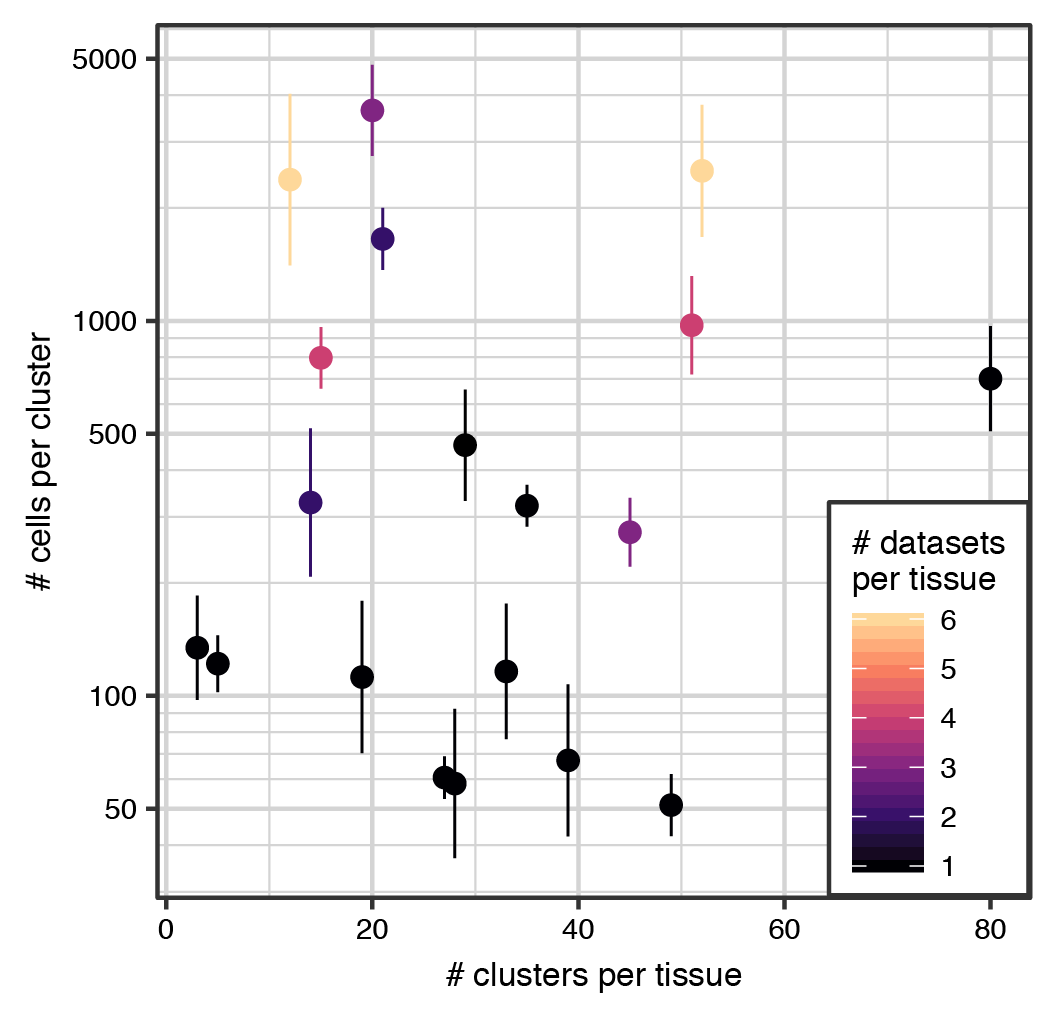
\includegraphics[scale=1.25]{Appendix2/Figs/tissue_cluster_dataset_numbers_HumanAtlas.png} % change word in curlies to change figure
\caption[Relating number of per-tissue clusters and number of cells]{\textbf{Relating number of per-tissue clusters and number of cells (Related to Figure~\ref{fig:chap4_HA}A)}\newline Scatter plot showing the variation of number of clusters per tissue with the number of cells, as well as number of datasets collected for each tissue (colour).}
\label{fig:appB_clustnumbs}
\end{figure}


\begin{figure}[ht!] 
\centering
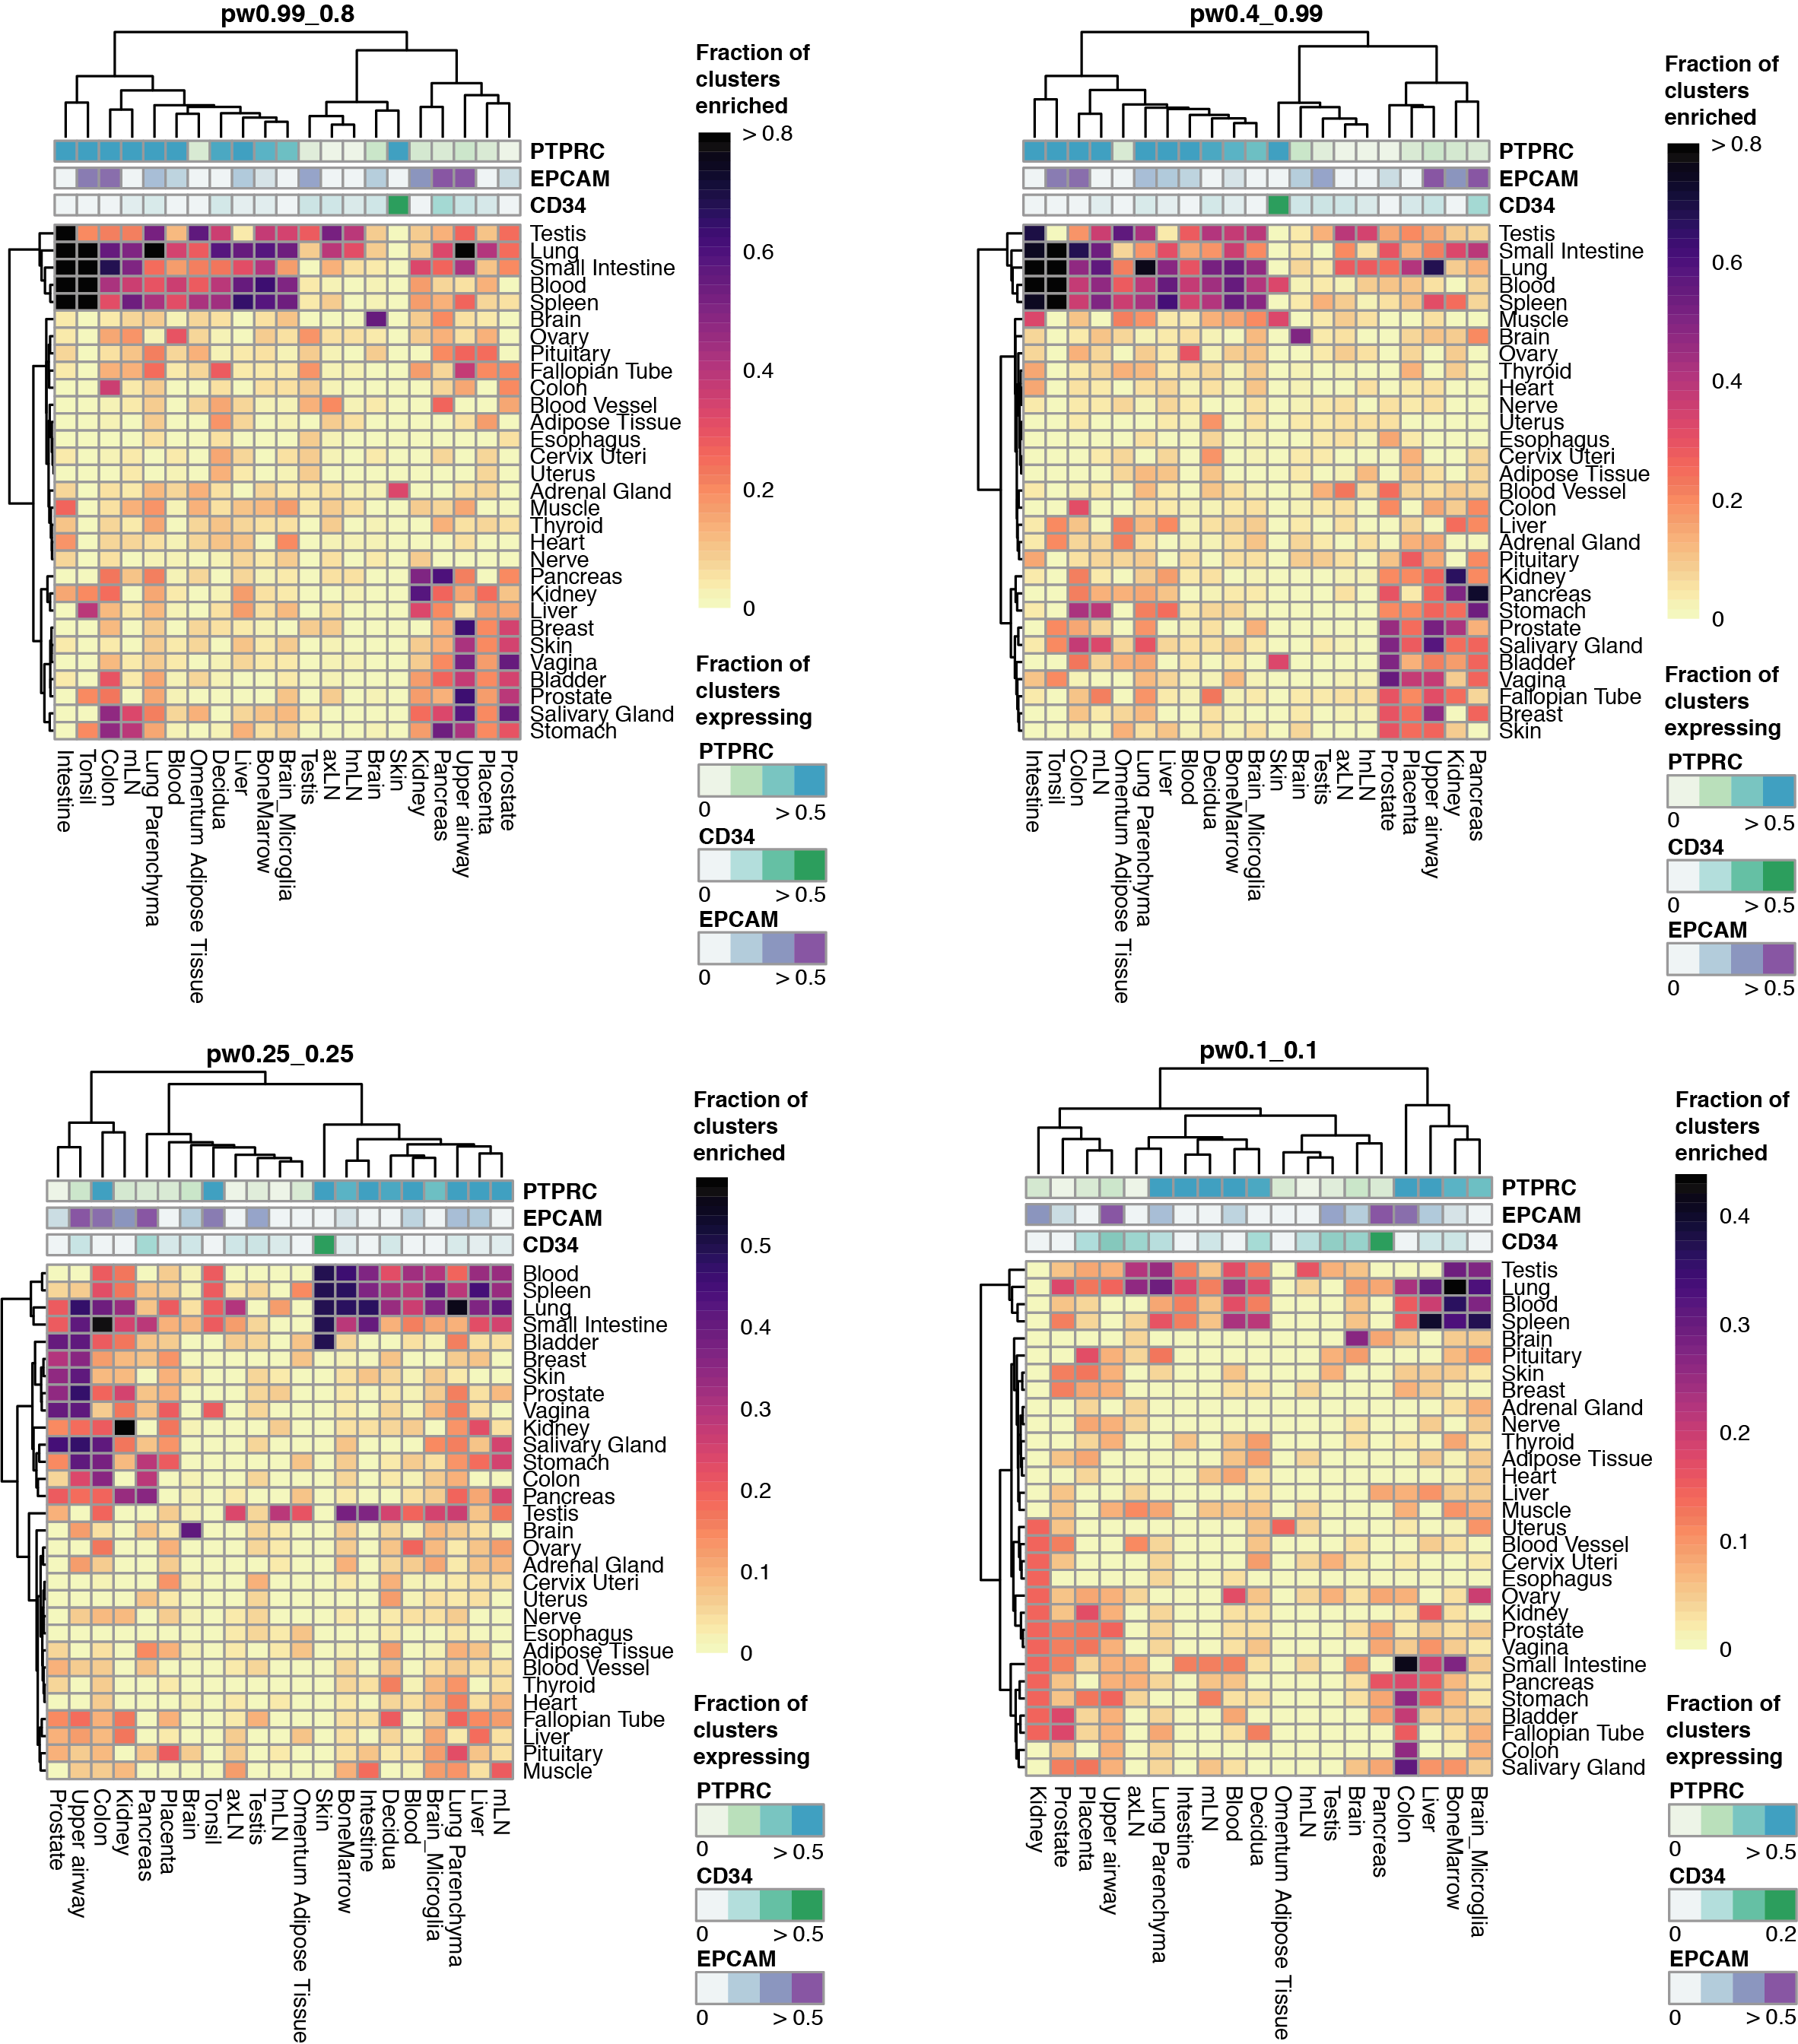
\includegraphics[scale=0.77]{Appendix2/Figs/appB_tissueGSEA.png} % change word in curlies to change figure
\caption[Enrichment of tissue gene modules in other \textit{CellTypist} models]{\textbf{Enrichment of tissue gene modules in other \textit{CellTypist} models (Related to Figure~\ref{fig:chap4_tiss})}\newline Heatmaps showing the fraction of clusters in each tissue (x-axis) with an enrichment for tissue-specific gene programmes (y-axis) determined from GTEx data. Each heatmap represents a different set of clusters per tissue, resulting from using different parameters in the \textit{CellTypist} pipeline. Plot for thr1 = 0.99, thr2 = 0.8 is identical to Figure~\ref{fig:chap4_tiss}B.}
\label{fig:appB_tissGSEA}
\end{figure}


\begin{figure}[ht!] 
\centering
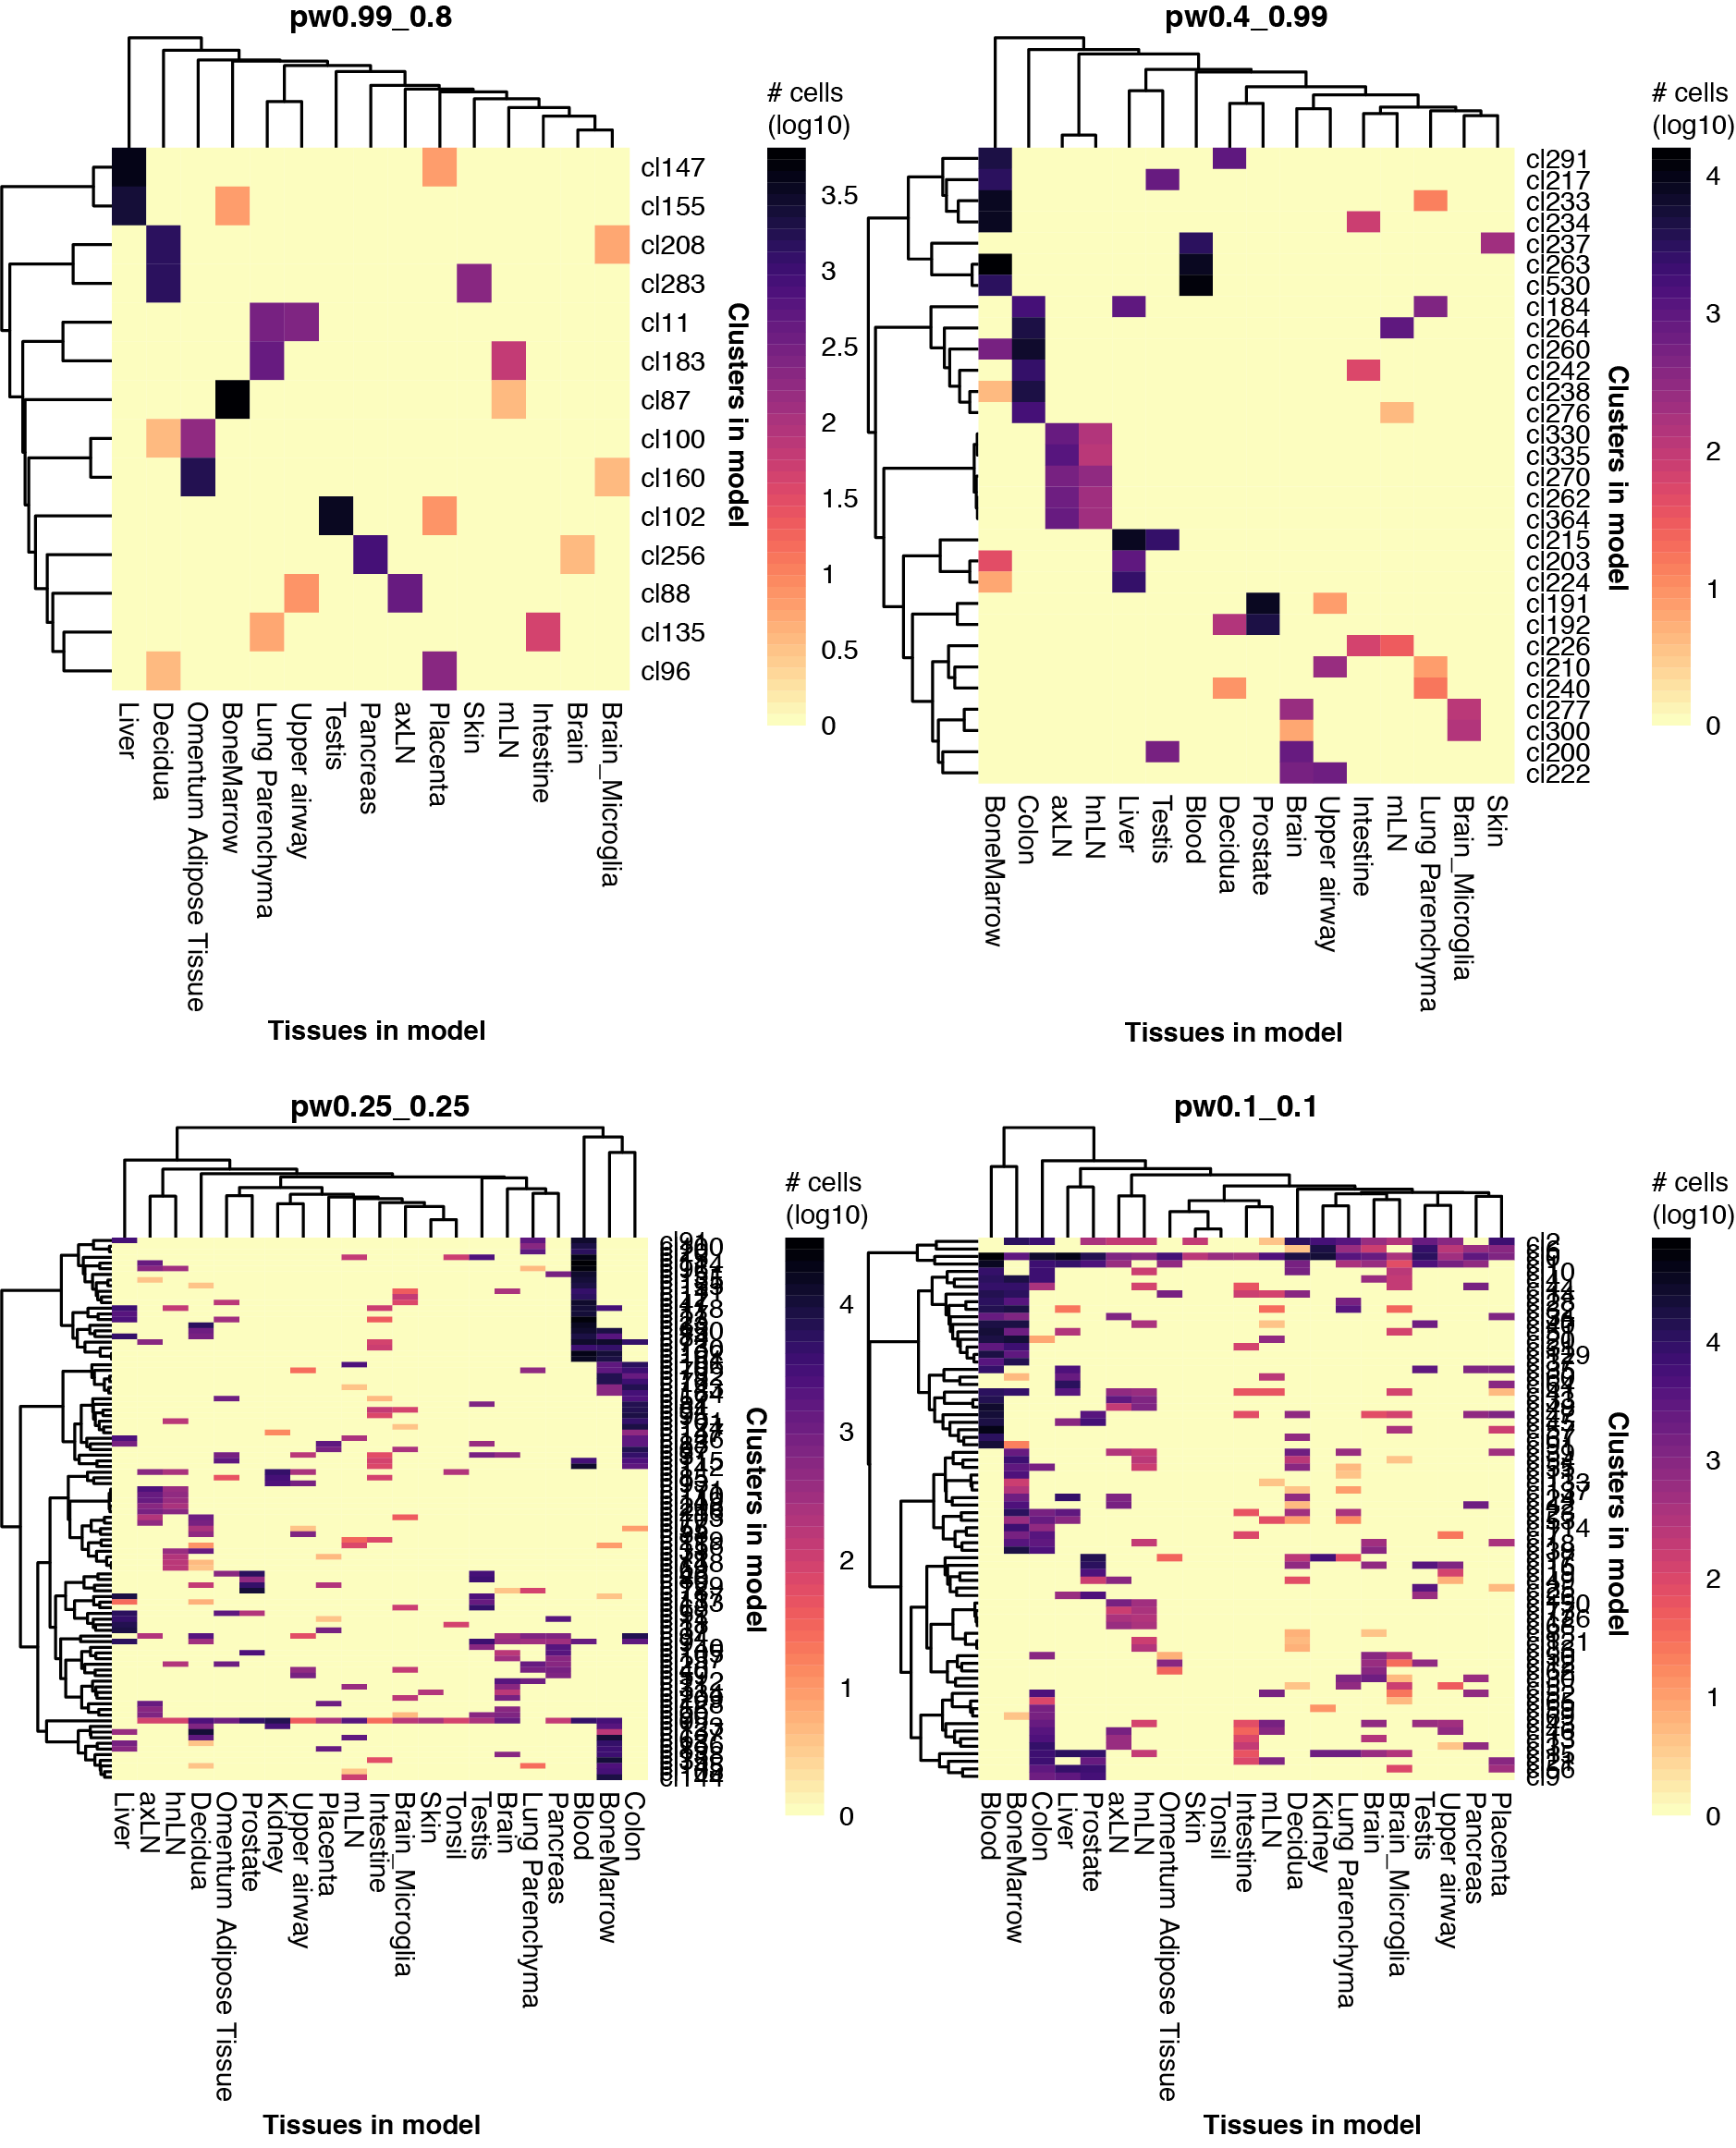
\includegraphics[width=1.0\textwidth]{Appendix2/Figs/appB_tissue_clustrelations_HumanAtlas.png} % change word in curlies to change figure
\caption[Clusters merged across tissues in the different models]{\textbf{Clusters merged across tissues in the different models (Related to Figure~\ref{fig:chap4_tiss})}\newline Heatmaps showing the number of cells contributed by each tissue into cross-tissue clusters for each model.}
\label{fig:appB_tissrel}
\end{figure}


\begin{figure}[ht!] 
\centering
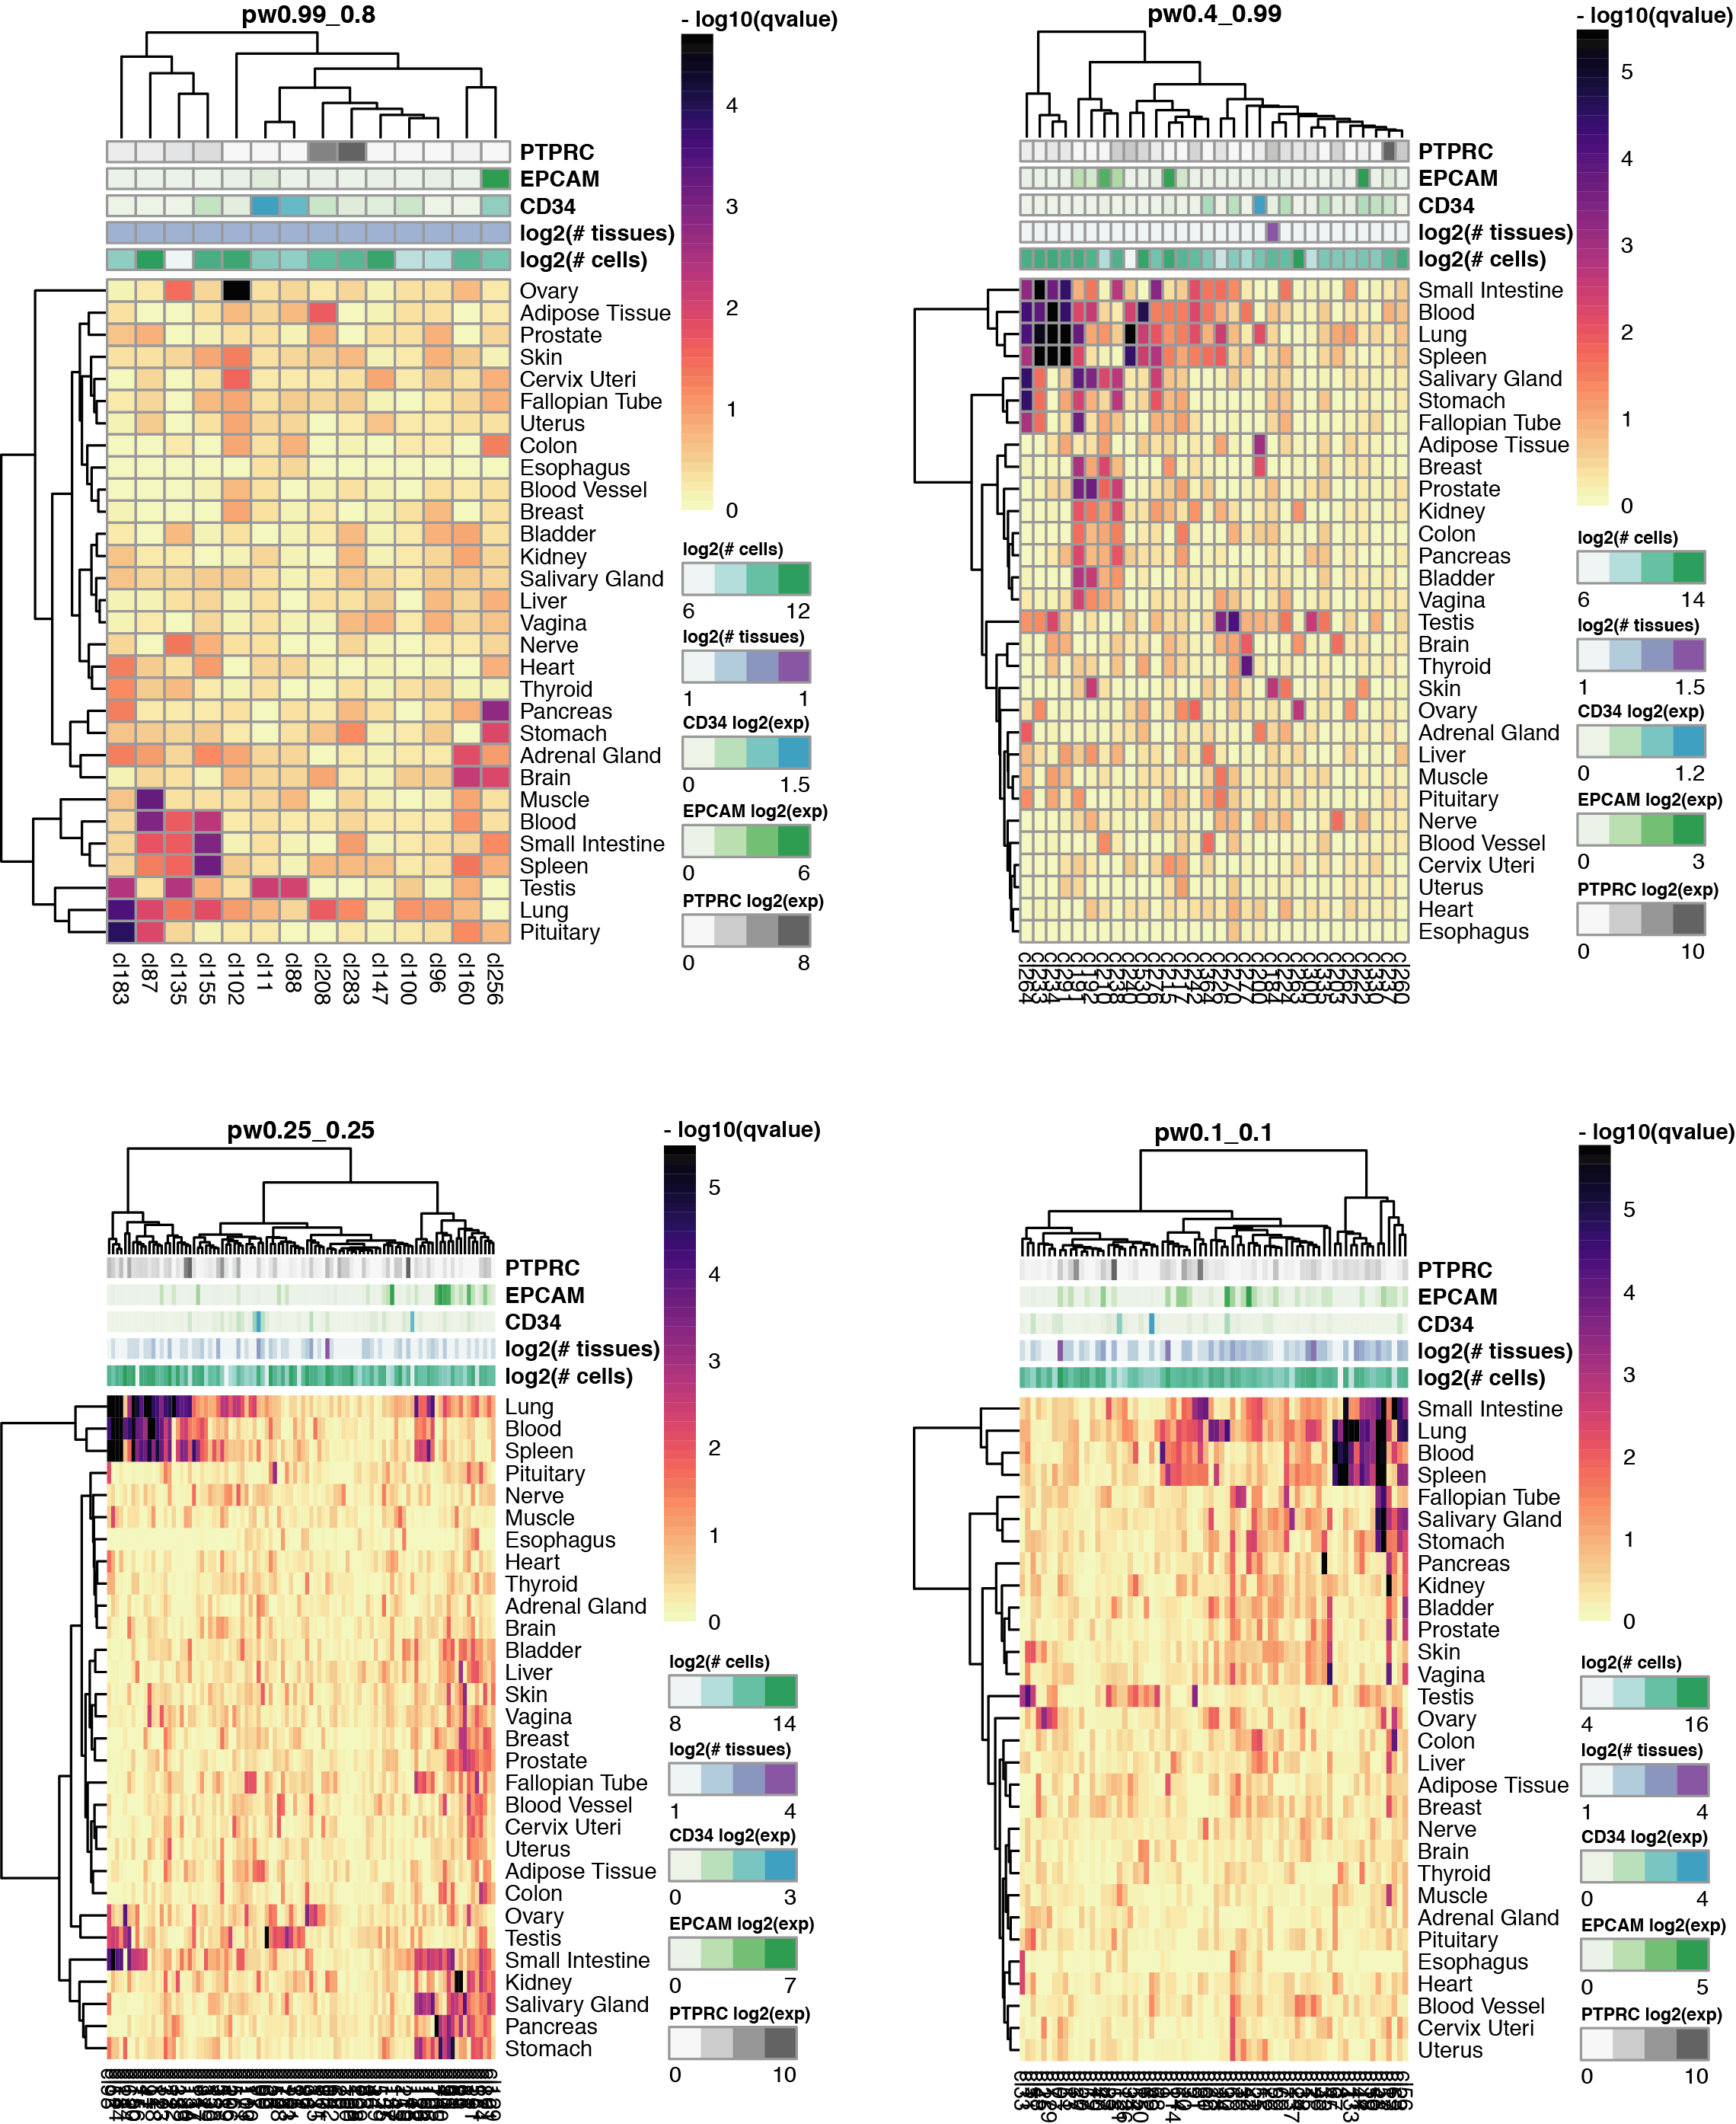
\includegraphics[scale=0.78]{Appendix2/Figs/appB_clmGSEA.png} % change word in curlies to change figure
\caption[Enrichment of tissue gene modules in merged clusters of different \textit{CellTypist} models]{\textbf{Enrichment of tissue gene modules in merged clusters of different \textit{CellTypist} models (Related to Figure~\ref{fig:chap4_tiss})}\newline Heatmaps showing the -log10(q-value) of each merged cluster (x-axis) for the enrichment of tissue-specific gene programmes (y-axis) in their top 500 genes output by the model. Each heatmap represents a different set of merged clusters, resulting from using different parameters in the \textit{CellTypist} pipeline.}
\label{fig:appB_clmGSEA}
\end{figure}


\begin{figure}[ht!] 
\centering
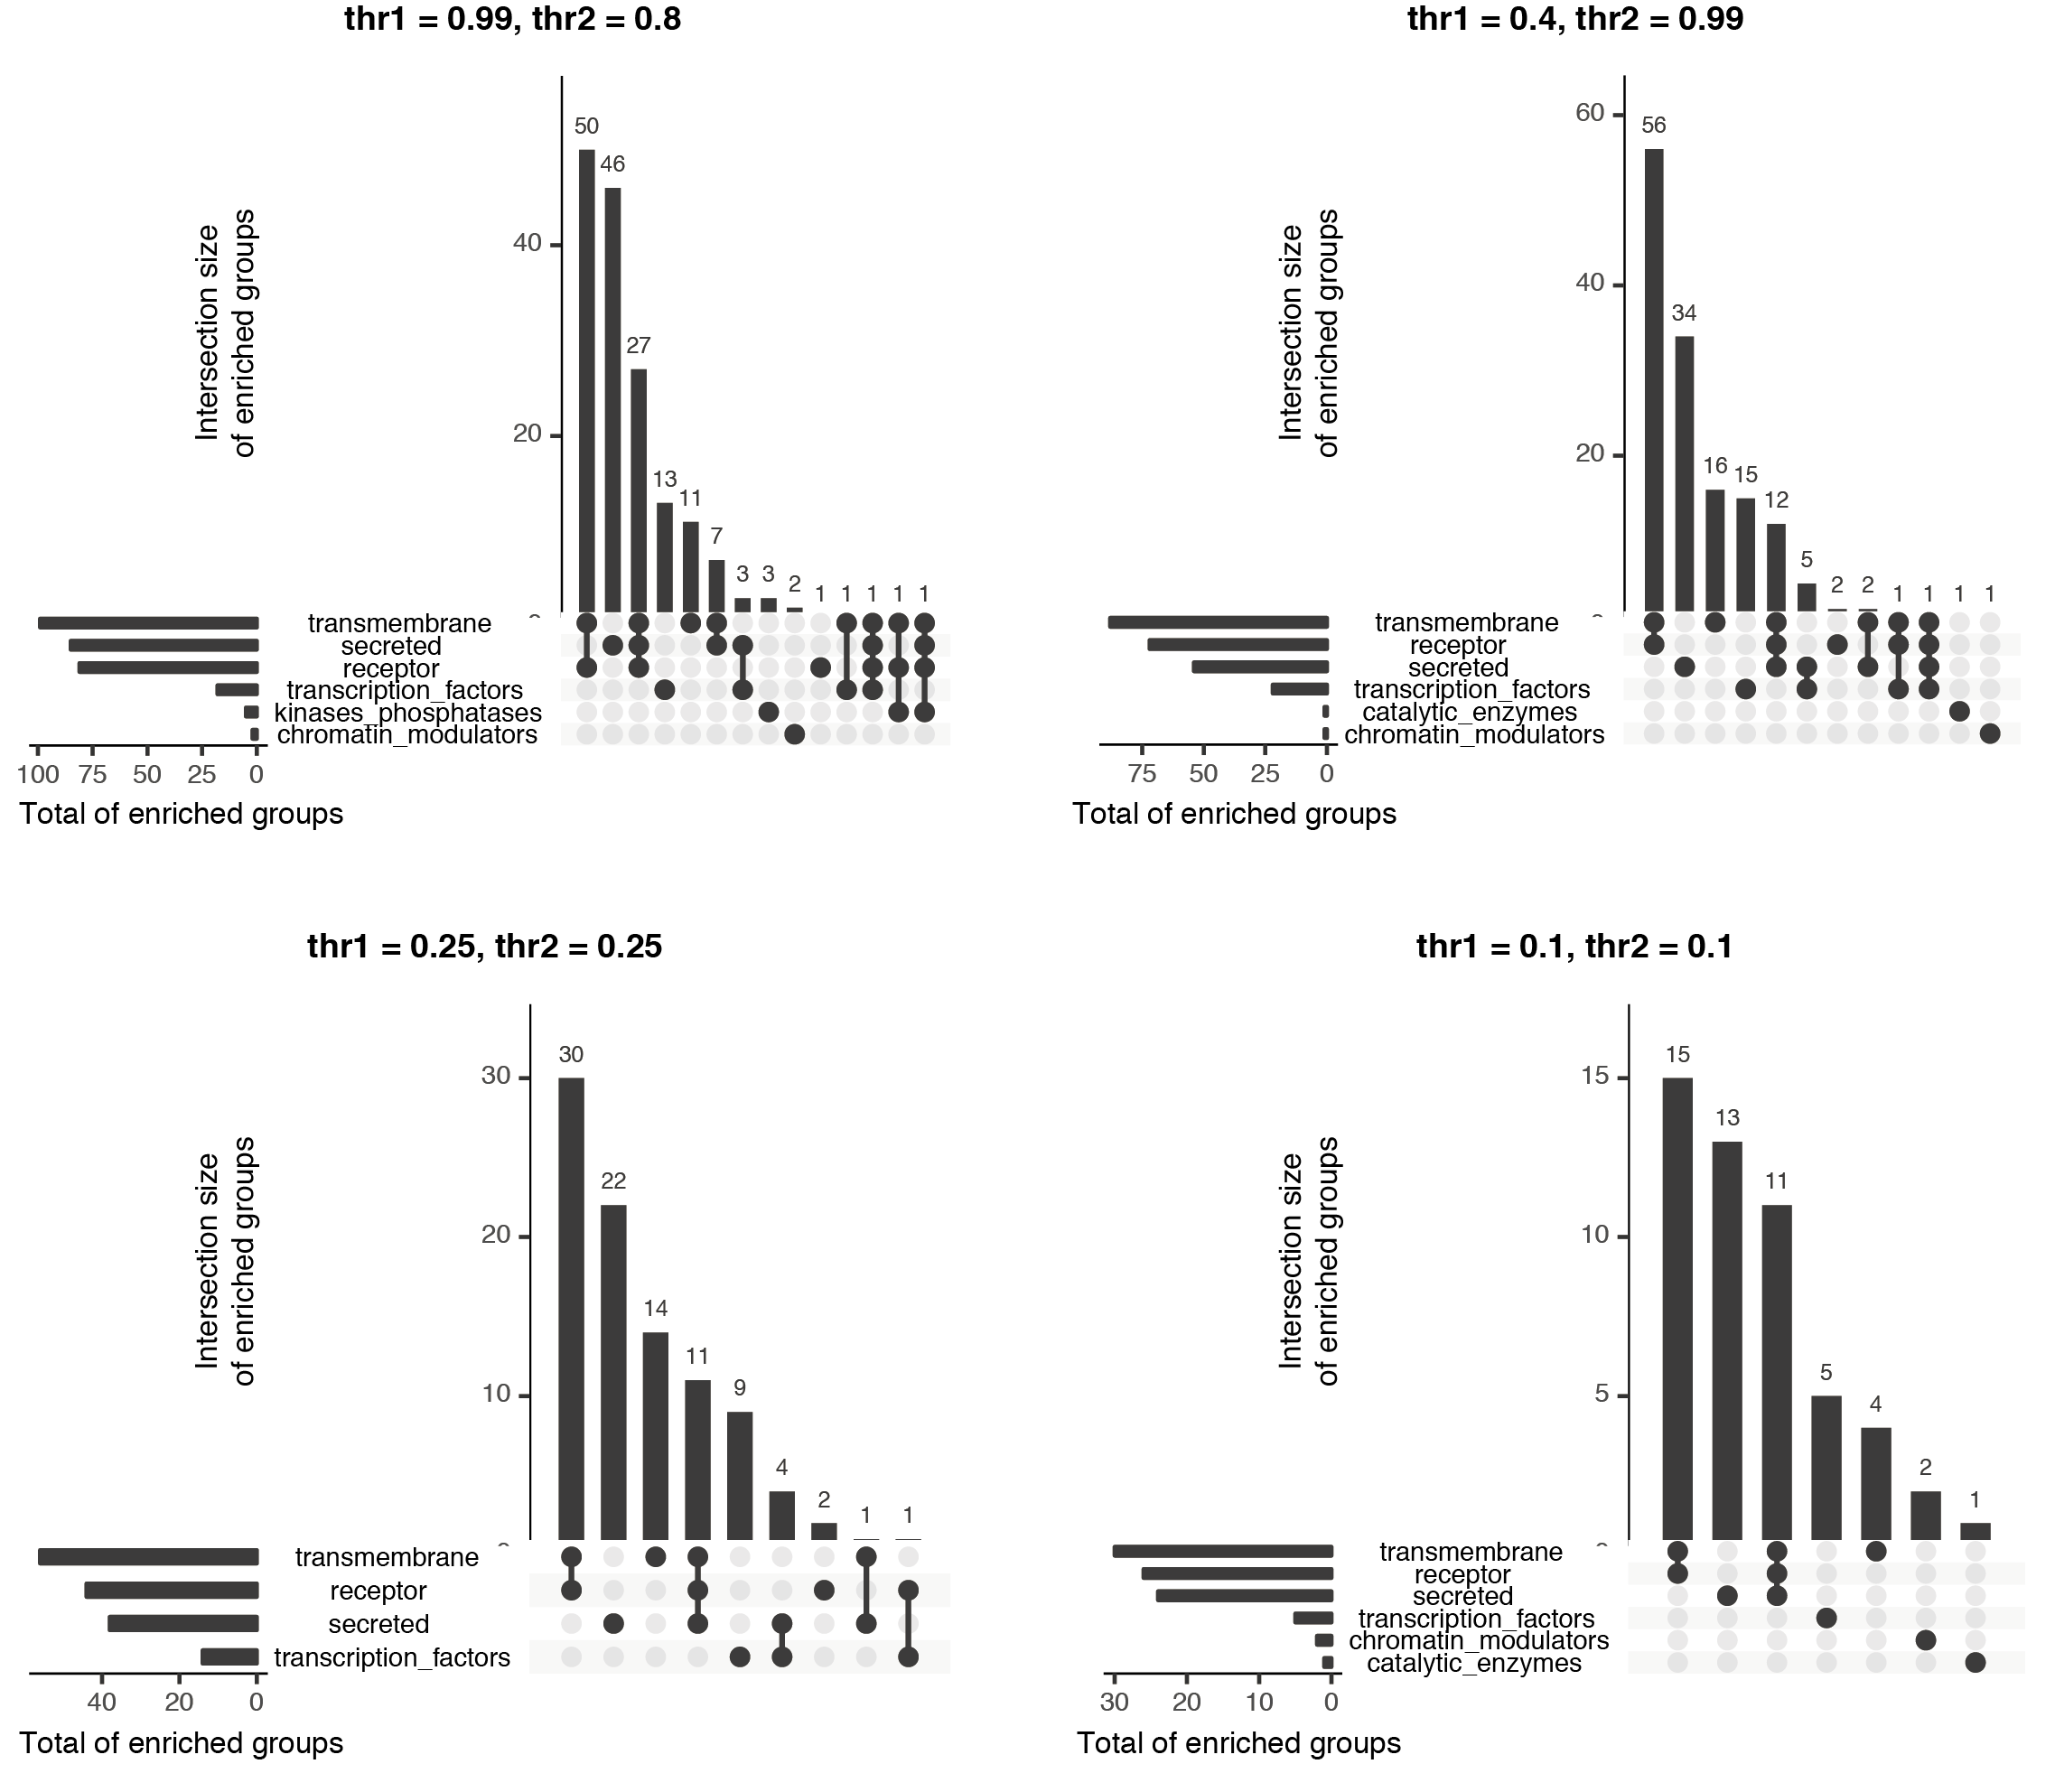
\includegraphics[scale=0.79]{Appendix2/Figs/appB_upset.png} % change word in curlies to change figure
\caption[Gene upset plots of different \textit{CellTypist} models]{\textbf{Gene upset plots of different \textit{CellTypist} models (Related to Figure~\ref{fig:chap4_genetypes})}\newline Upset plots counting the number of clusters enriched for a specific group of genes in each model. The gene groups tested were "transcription factors", "transmembrane", "secreted", "receptors", "membrane peripheral proteins", "kinases and phosphatases", "chromatin modulators", "catalytic enzymes", "housekeeping genes". Only the terms enriched in at least one cluster were shown. The plot for thr1 = 0.99, thr2 = 0.8 is identical to Figure~\ref{fig:chap4_genetypes}B.}
\label{fig:appB_supupset}
\end{figure}


\begin{figure}[pht!] 
\centering
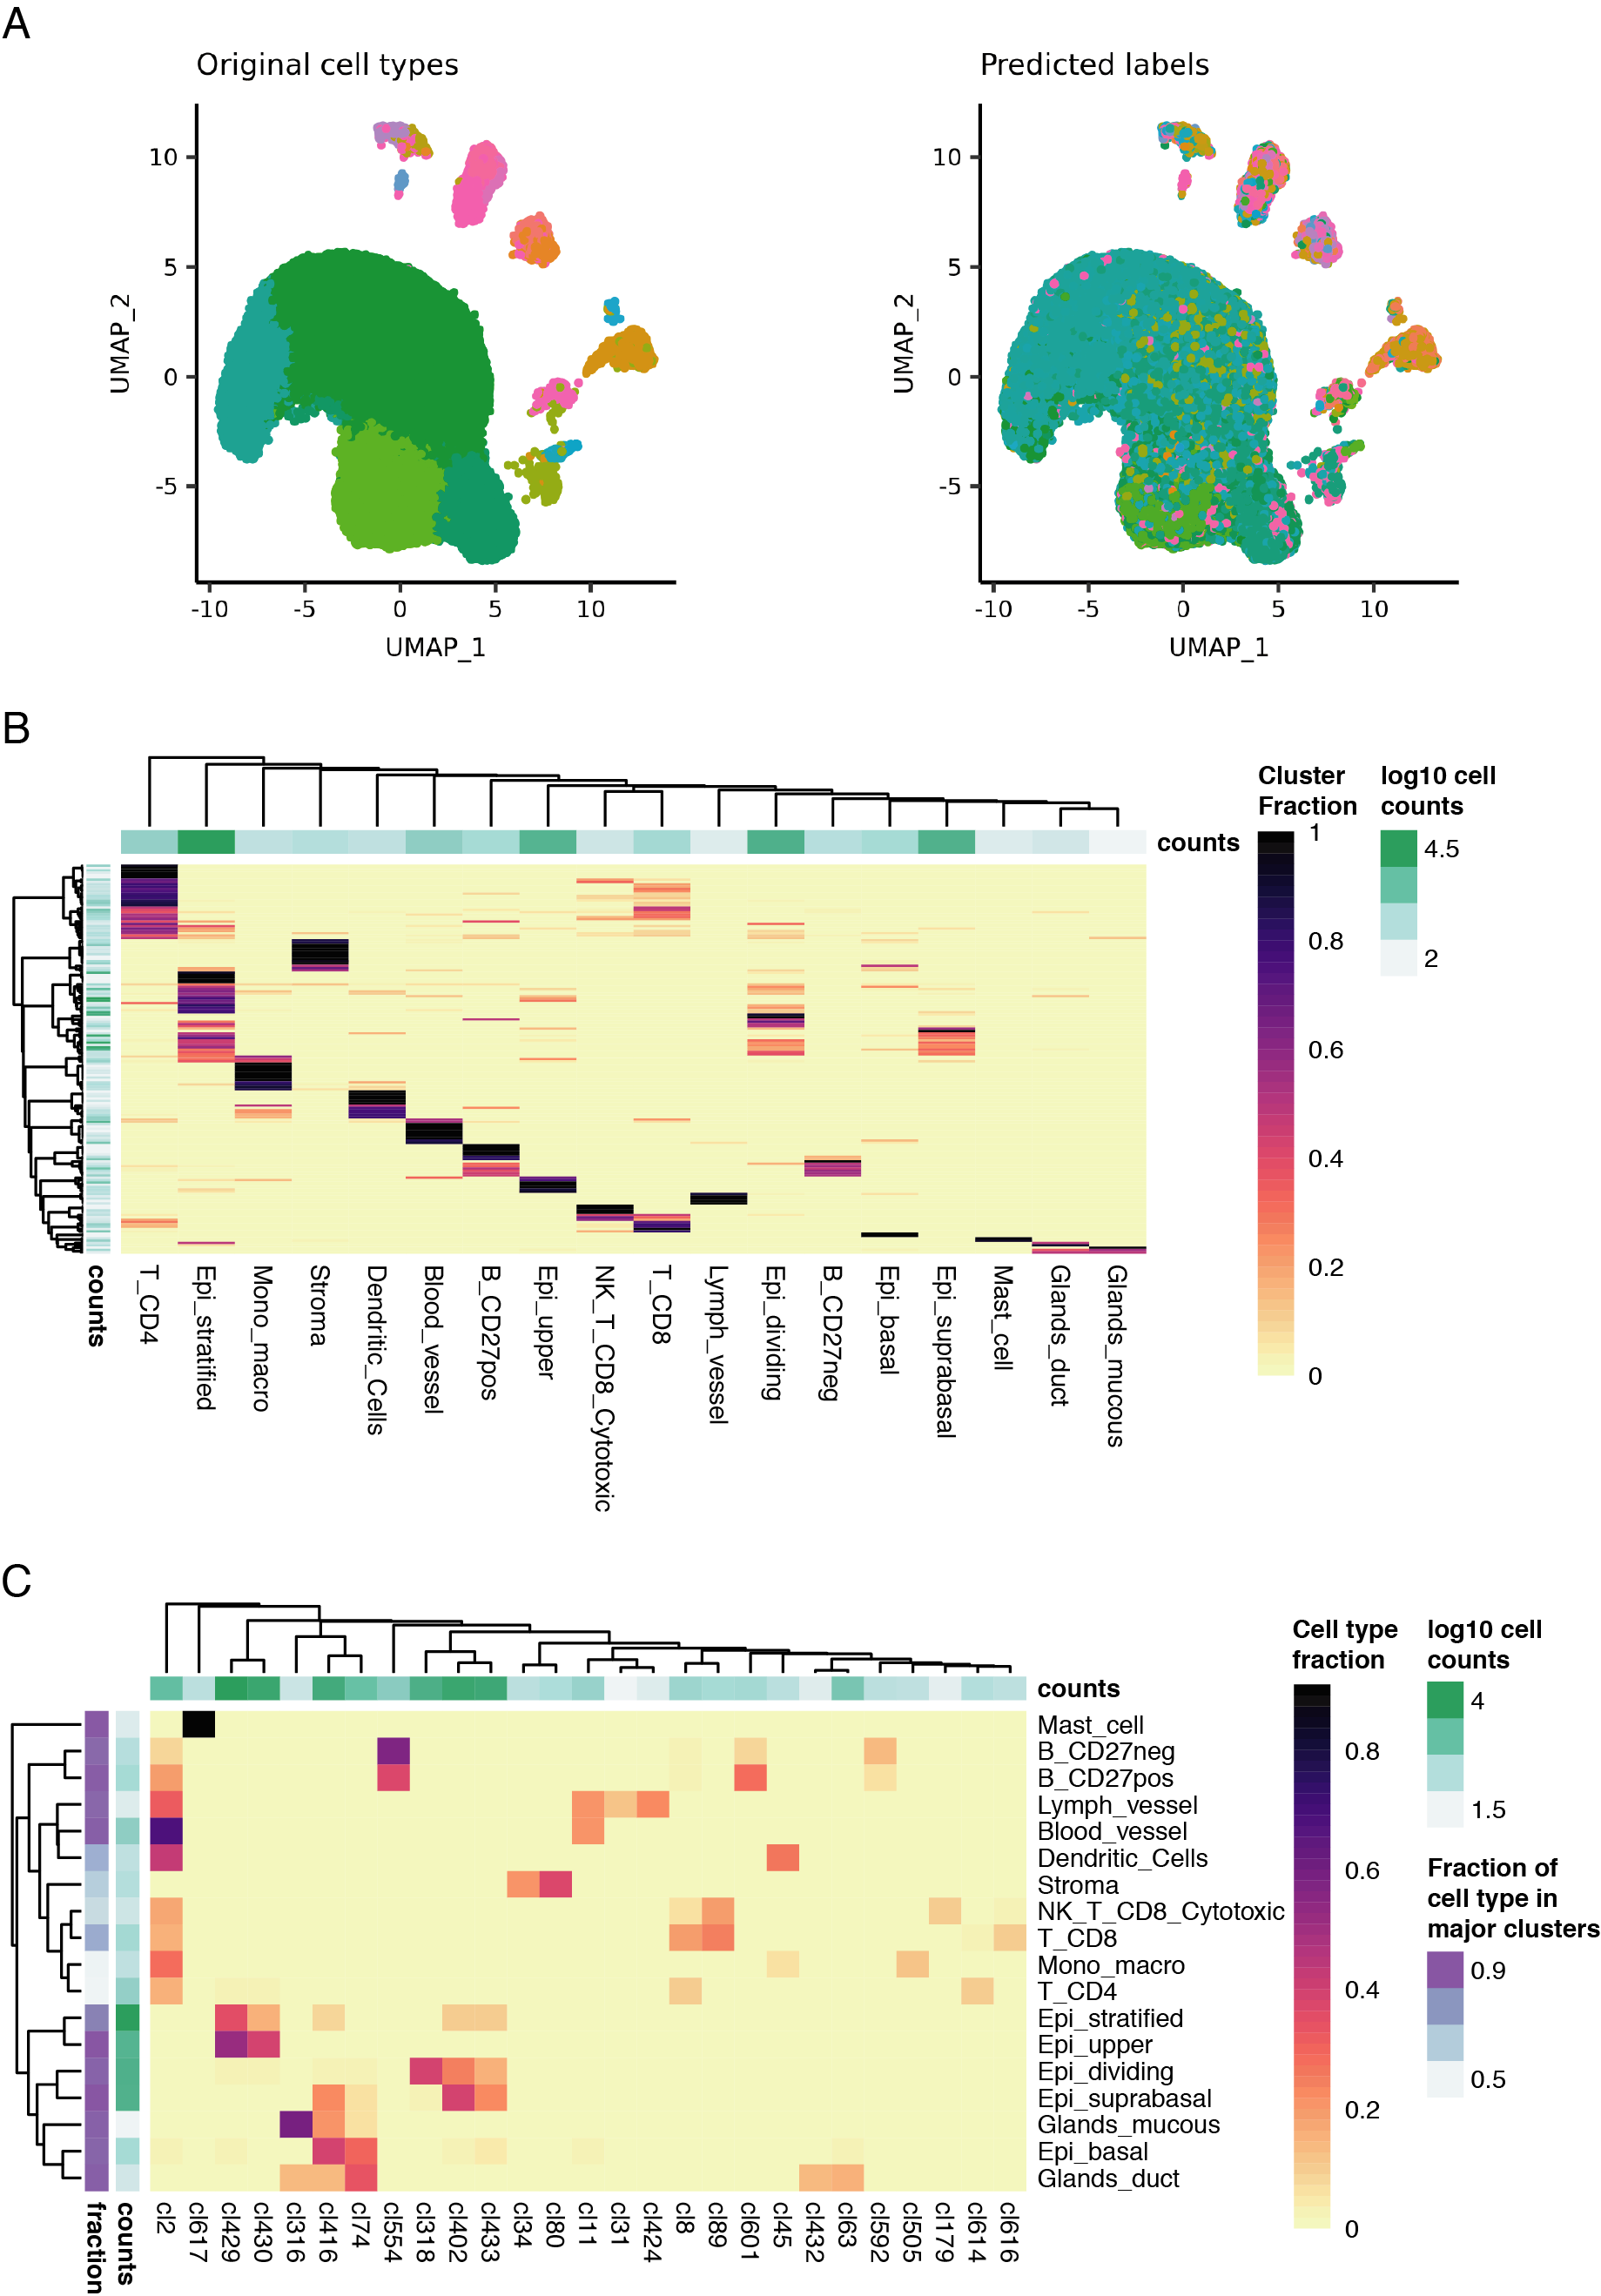
\includegraphics[scale=0.8]{Appendix2/Figs/appB_oes.png} % change word in curlies to change figure
\caption[\textit{CellTypist} predictions for oesophagus data from~\citep{madissoon_lung_2019}]{\textbf{\textit{CellTypist} predictions for oesophagus data from~\citep{madissoon_lung_2019} (Related to Figure~\ref{fig:chap4_preds})}\newline\textbf{(A)} UMAP projections coloured by the original cell type annotations (left) and those predicted by \textit{CellTypist} (right) using thr1 = 0.99 and thr2 = 0.8. \textbf{(B)} Proportion of clusters (rows) matching each annotated cell type (columns). \textbf{(C)} Proportion of annotated cell types (rows) included in each cluster (columns). Only clusters including at least 10\% of a given cell type were included.}
\label{fig:appB_oes}
\end{figure}


\begin{figure}[pht!] 
\centering
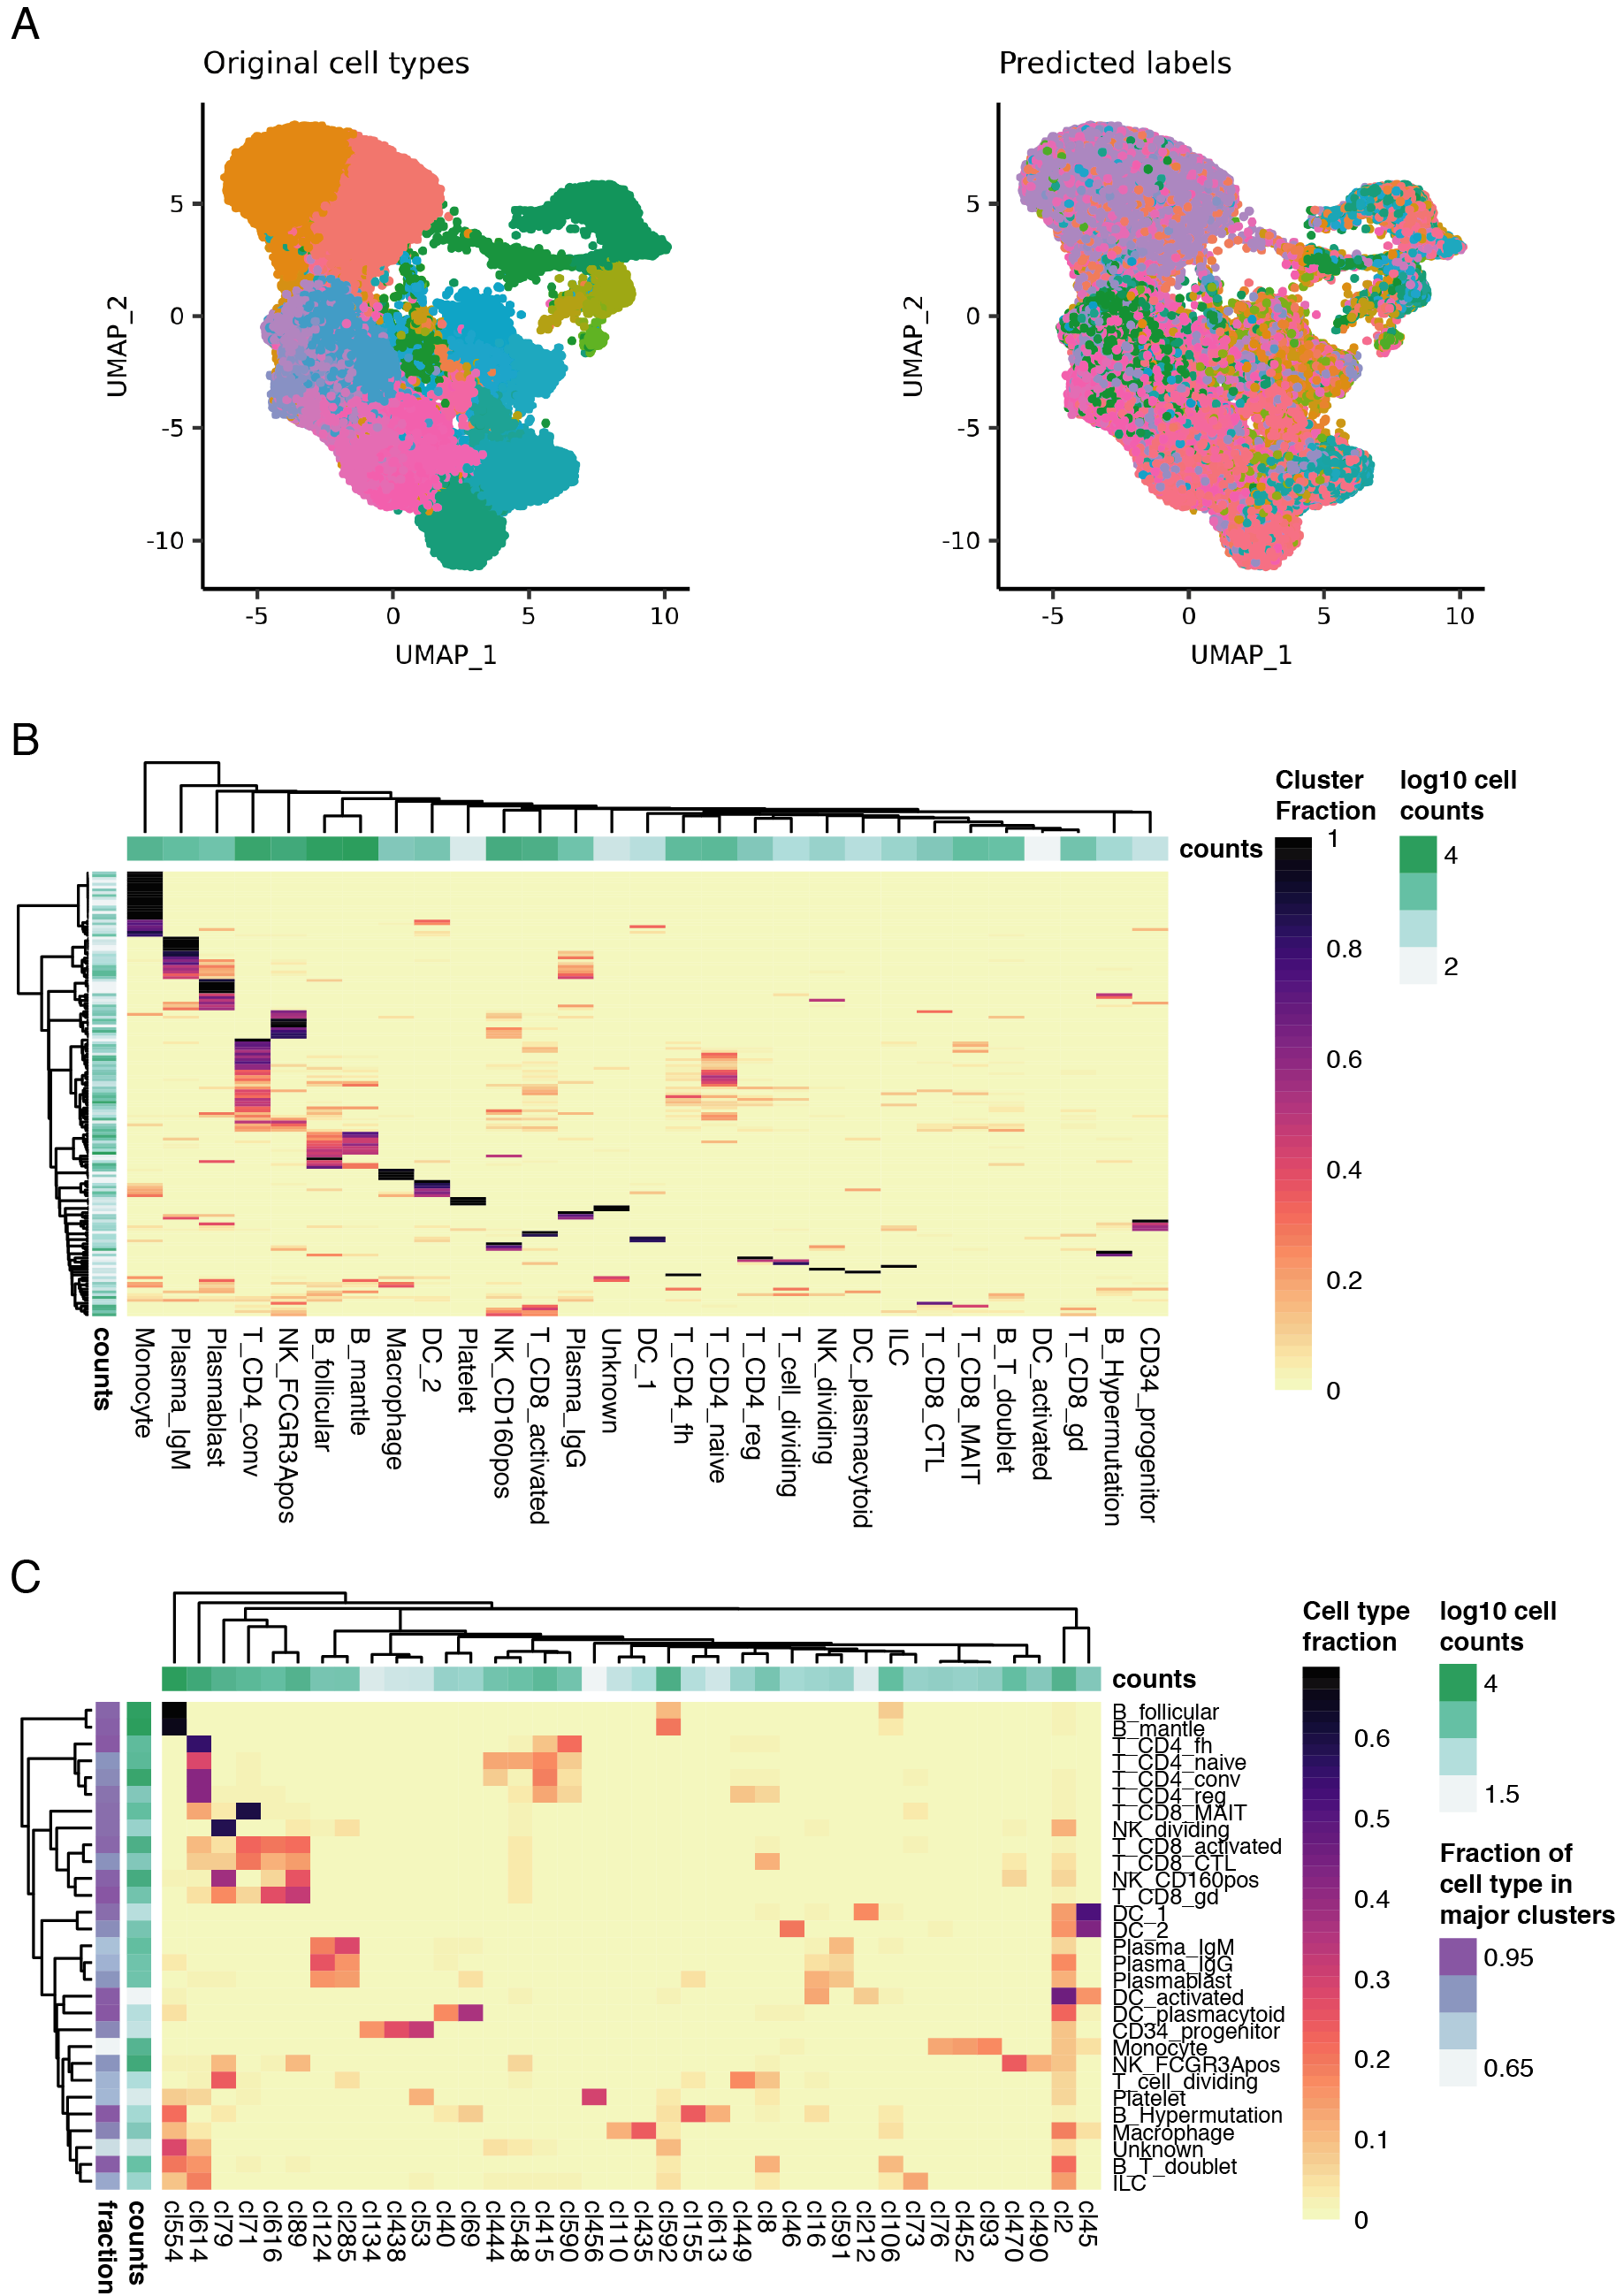
\includegraphics[scale=0.81]{Appendix2/Figs/appB_spleen.png} % change word in curlies to change figure
\caption[\textit{CellTypist} predictions for spleen data from~\citep{madissoon_lung_2019}]{\textbf{\textit{CellTypist} predictions for spleen data from~\citep{madissoon_lung_2019} (Related to Figure~\ref{fig:chap4_preds})}\newline\textbf{(A)} UMAP projections coloured by the original cell type annotations (left) and those predicted by \textit{CellTypist} (right) using thr1 = 0.99 and thr2 = 0.8. \textbf{(B)} Proportion of clusters (rows) matching each annotated cell type (columns). \textbf{(C)} Proportion of annotated cell types (rows) included in each cluster (columns). Only clusters including at least 10\% of a given cell type were included.}
\label{fig:appB_spleen}
\end{figure}


\begin{figure}[pht!] 
\centering
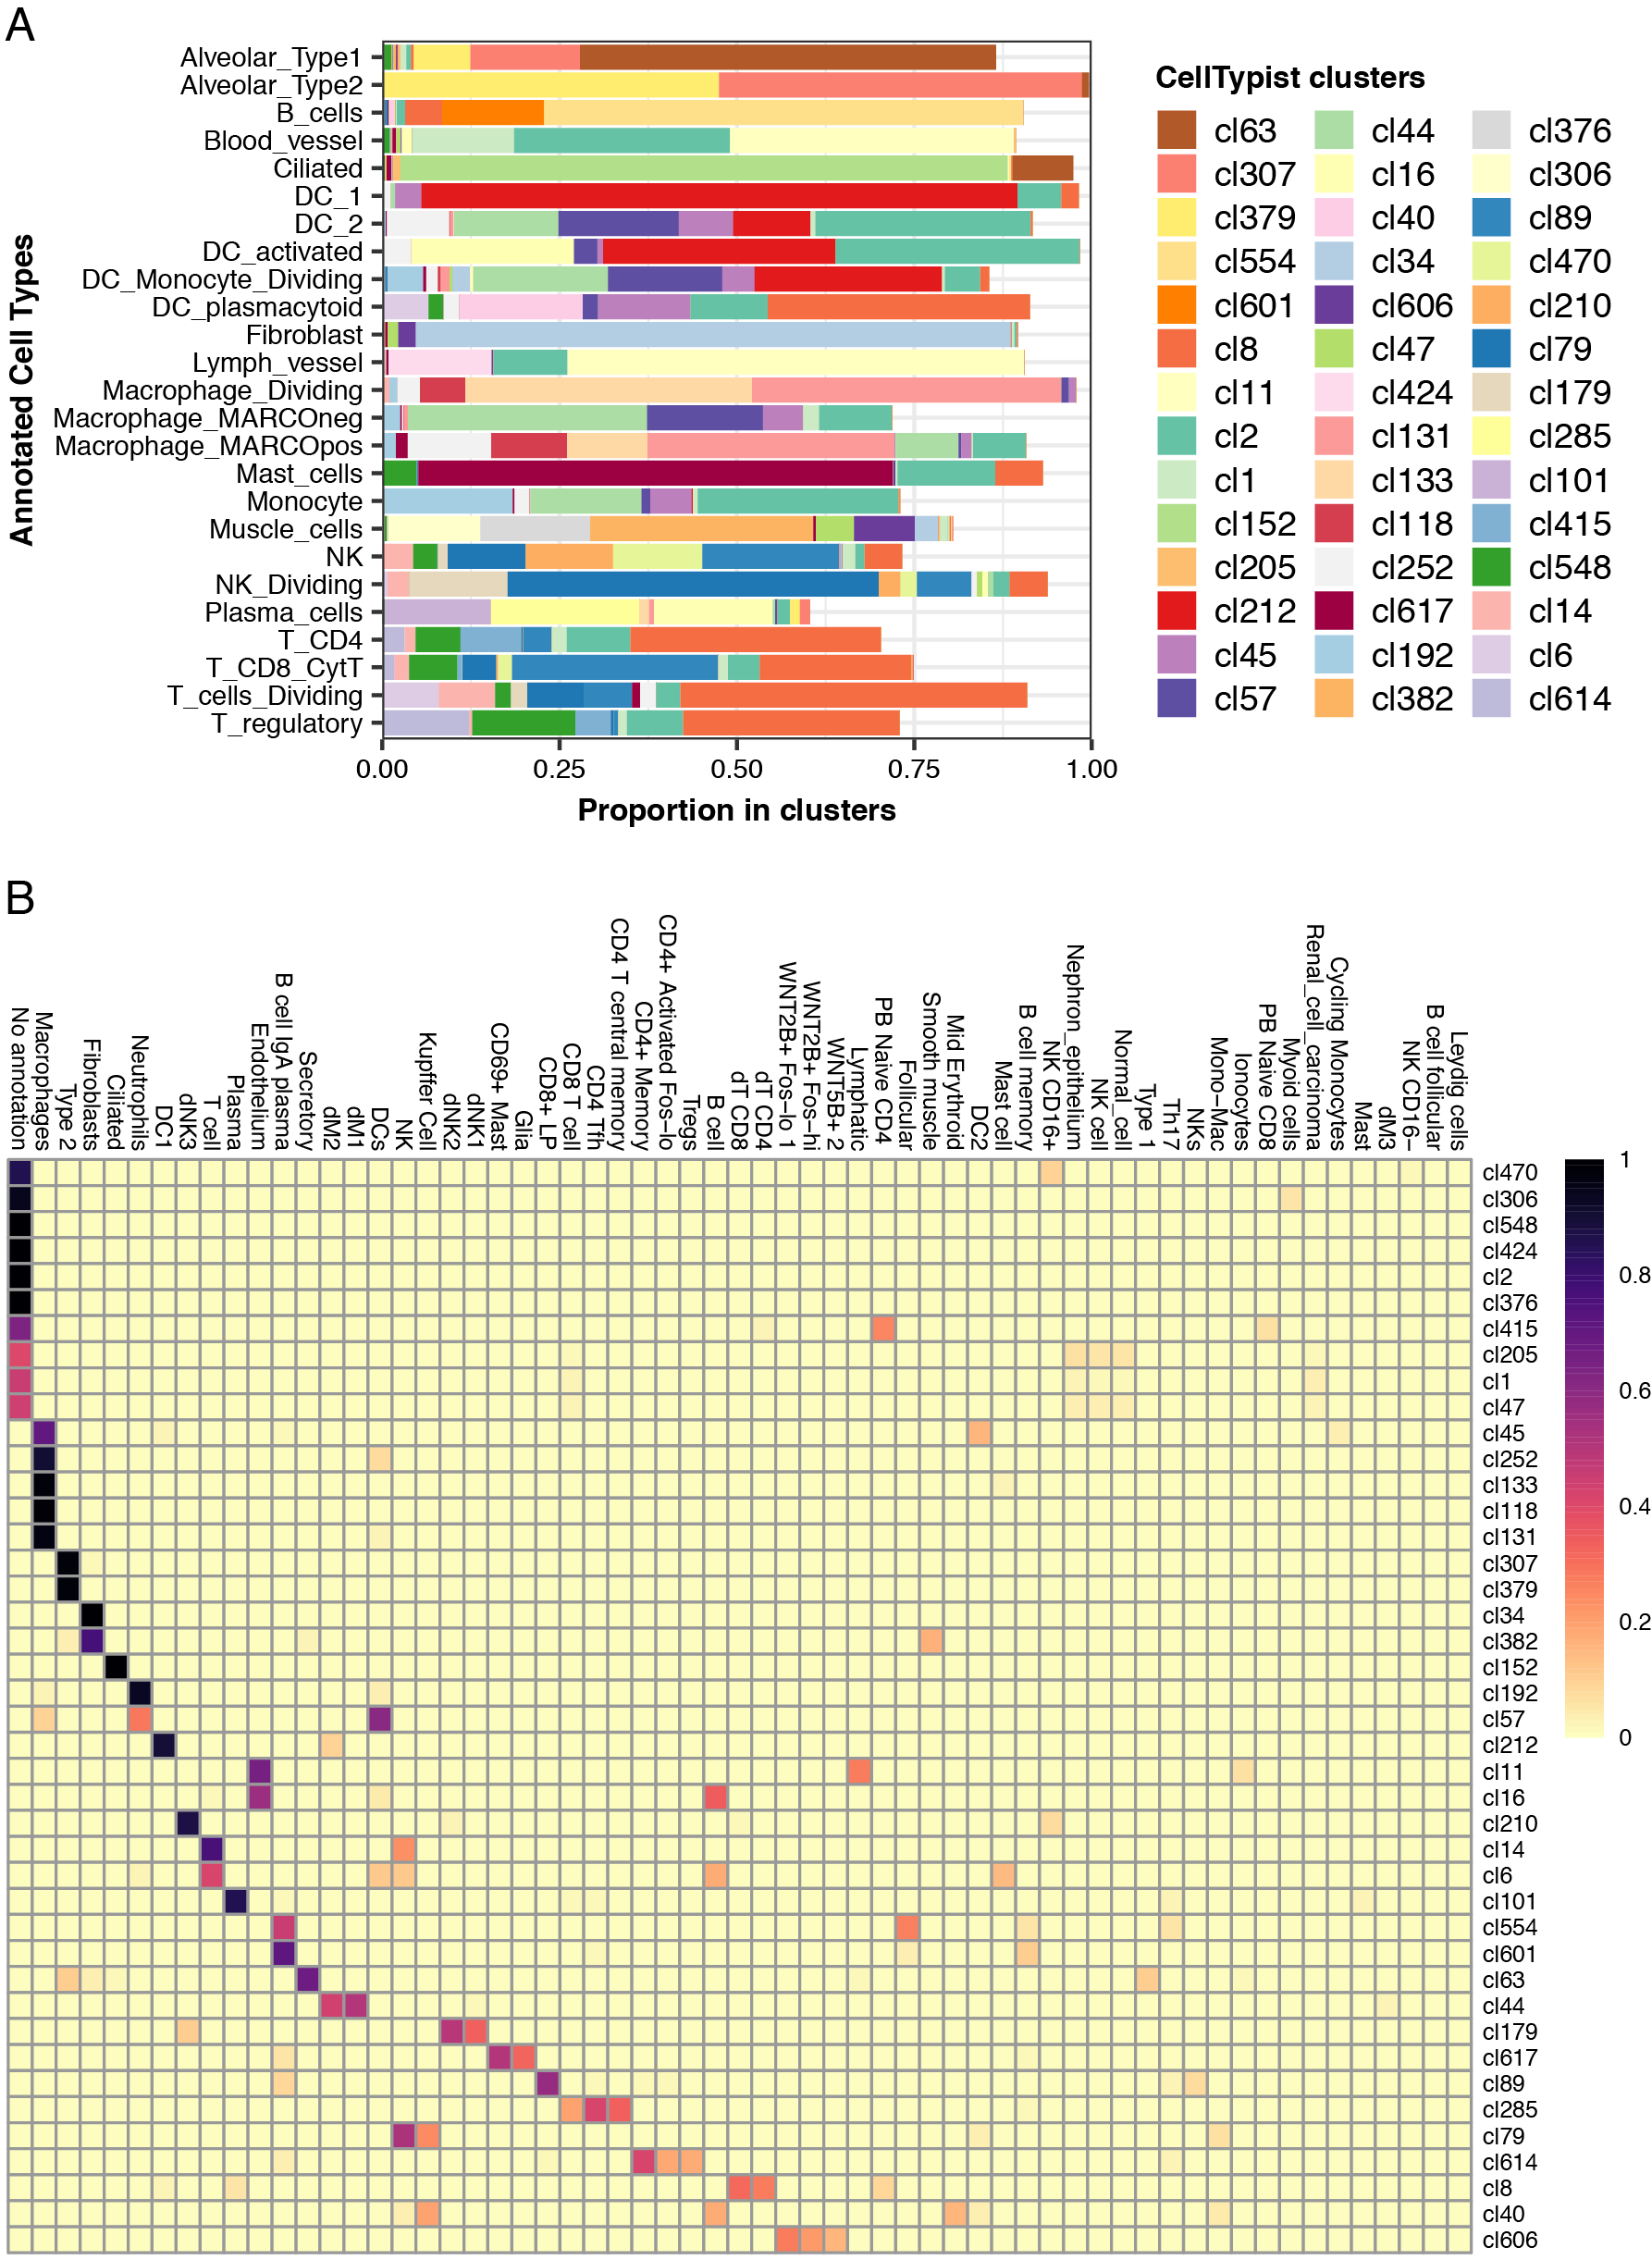
\includegraphics[scale=0.93]{Appendix2/Figs/appB_lung_labs_exp.png} % change word in curlies to change figure
\caption[Matching \textit{CellTypist} predictions in lung with annotations in the data collection]{\textbf{Matching \textit{CellTypist} predictions in lung with annotations in the data collection (Related to Figure~\ref{fig:chap4_preds})}\newline\textbf{(A)} \textit{CellTypist} clusters (thr1 = 0.99, thr2 = 0.8) matched to each original cell type annotation. Only the top 3 clusters per cell type were selected. \textbf{(B)} Proportion of cell type annotations (columns) represented in the \textit{CellTypist} clusters matched to lung.}
\label{fig:appB_lunglabs}
\end{figure}


\begin{figure}[ht!] 
\centering
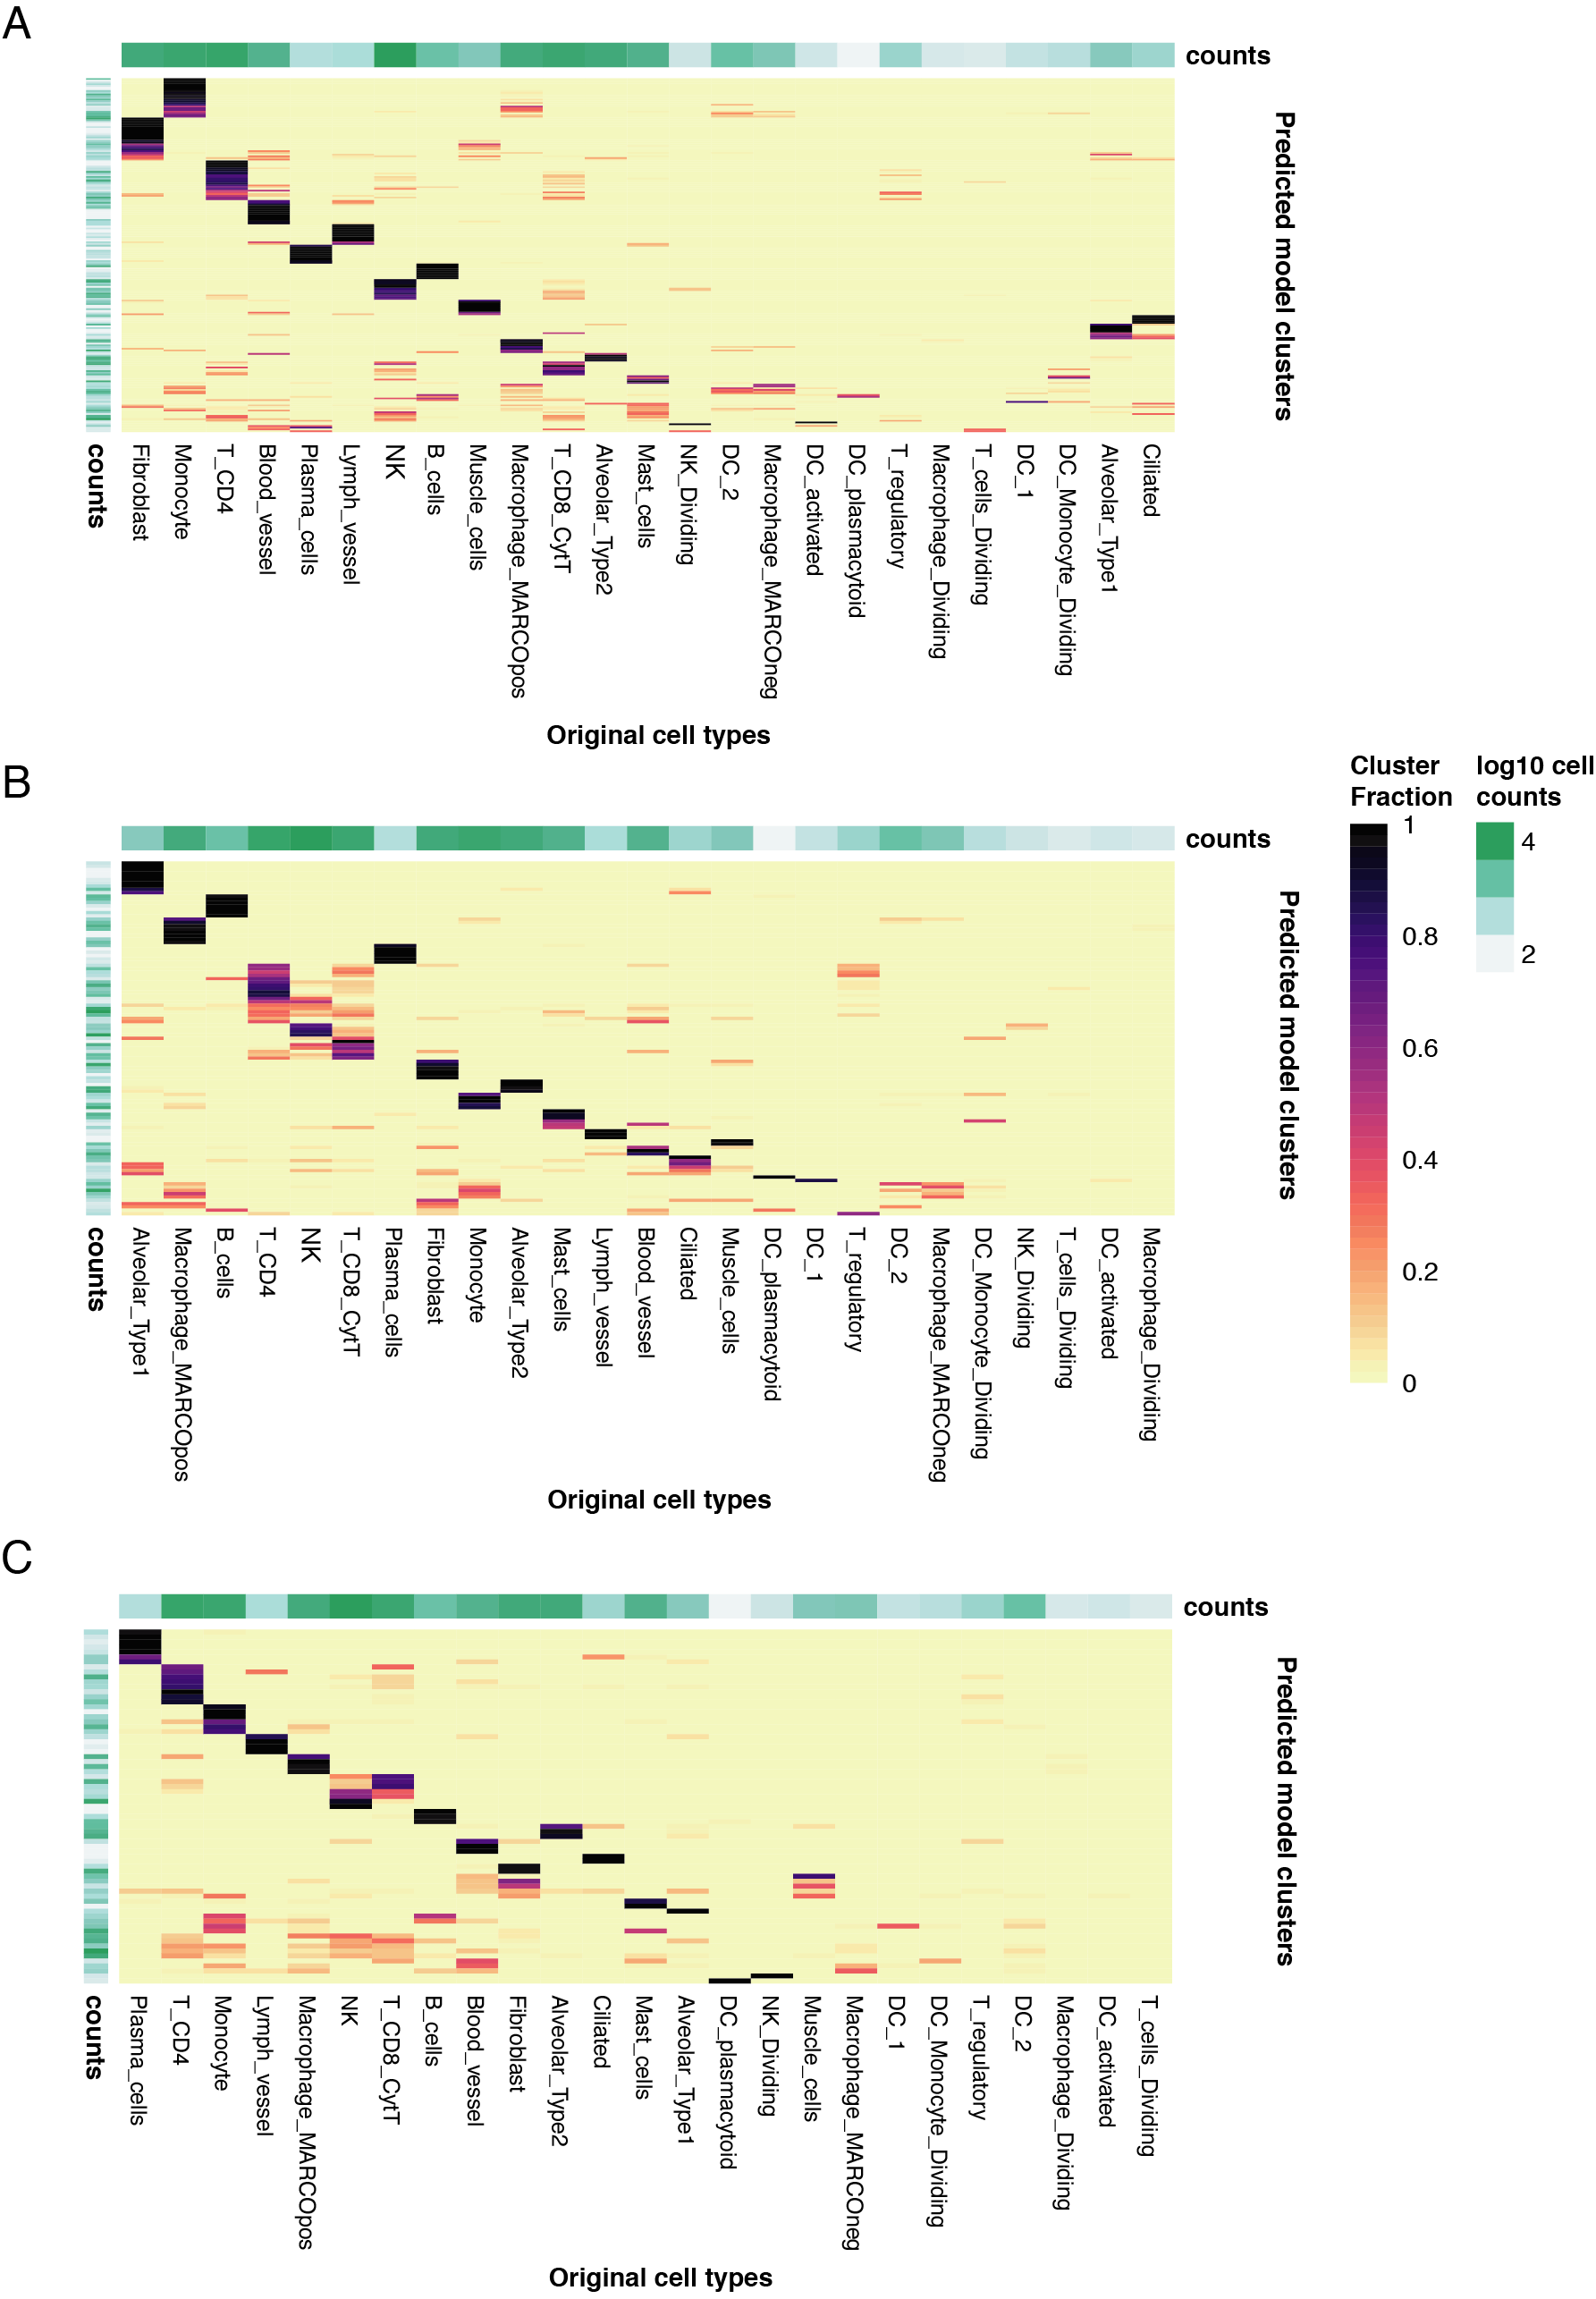
\includegraphics[scale=0.85]{Appendix2/Figs/appB_otherClustFrac_lung.png} % change word in curlies to change figure
\caption[Clusters matching lung annotated cell types in other \textit{CellTypist} models]{\textbf{Clusters matching lung annotated cell types in other \textit{CellTypist} models (Related to Figure~\ref{fig:chap4_preds}B)}\newline Proportion of clusters (rows) matching each annotated cell type (columns) in the models thr1 = 0.4, thr2 = 0.99 \textbf{(A)}, thr1 = 0.25, thr2 = 0.25 \textbf{(A)}, and thr1 = 0.1, thr2 = 0.1 \textbf{(C)}.}
\label{fig:appB_othercl}
\end{figure}


\begin{figure}[ht!] 
\centering
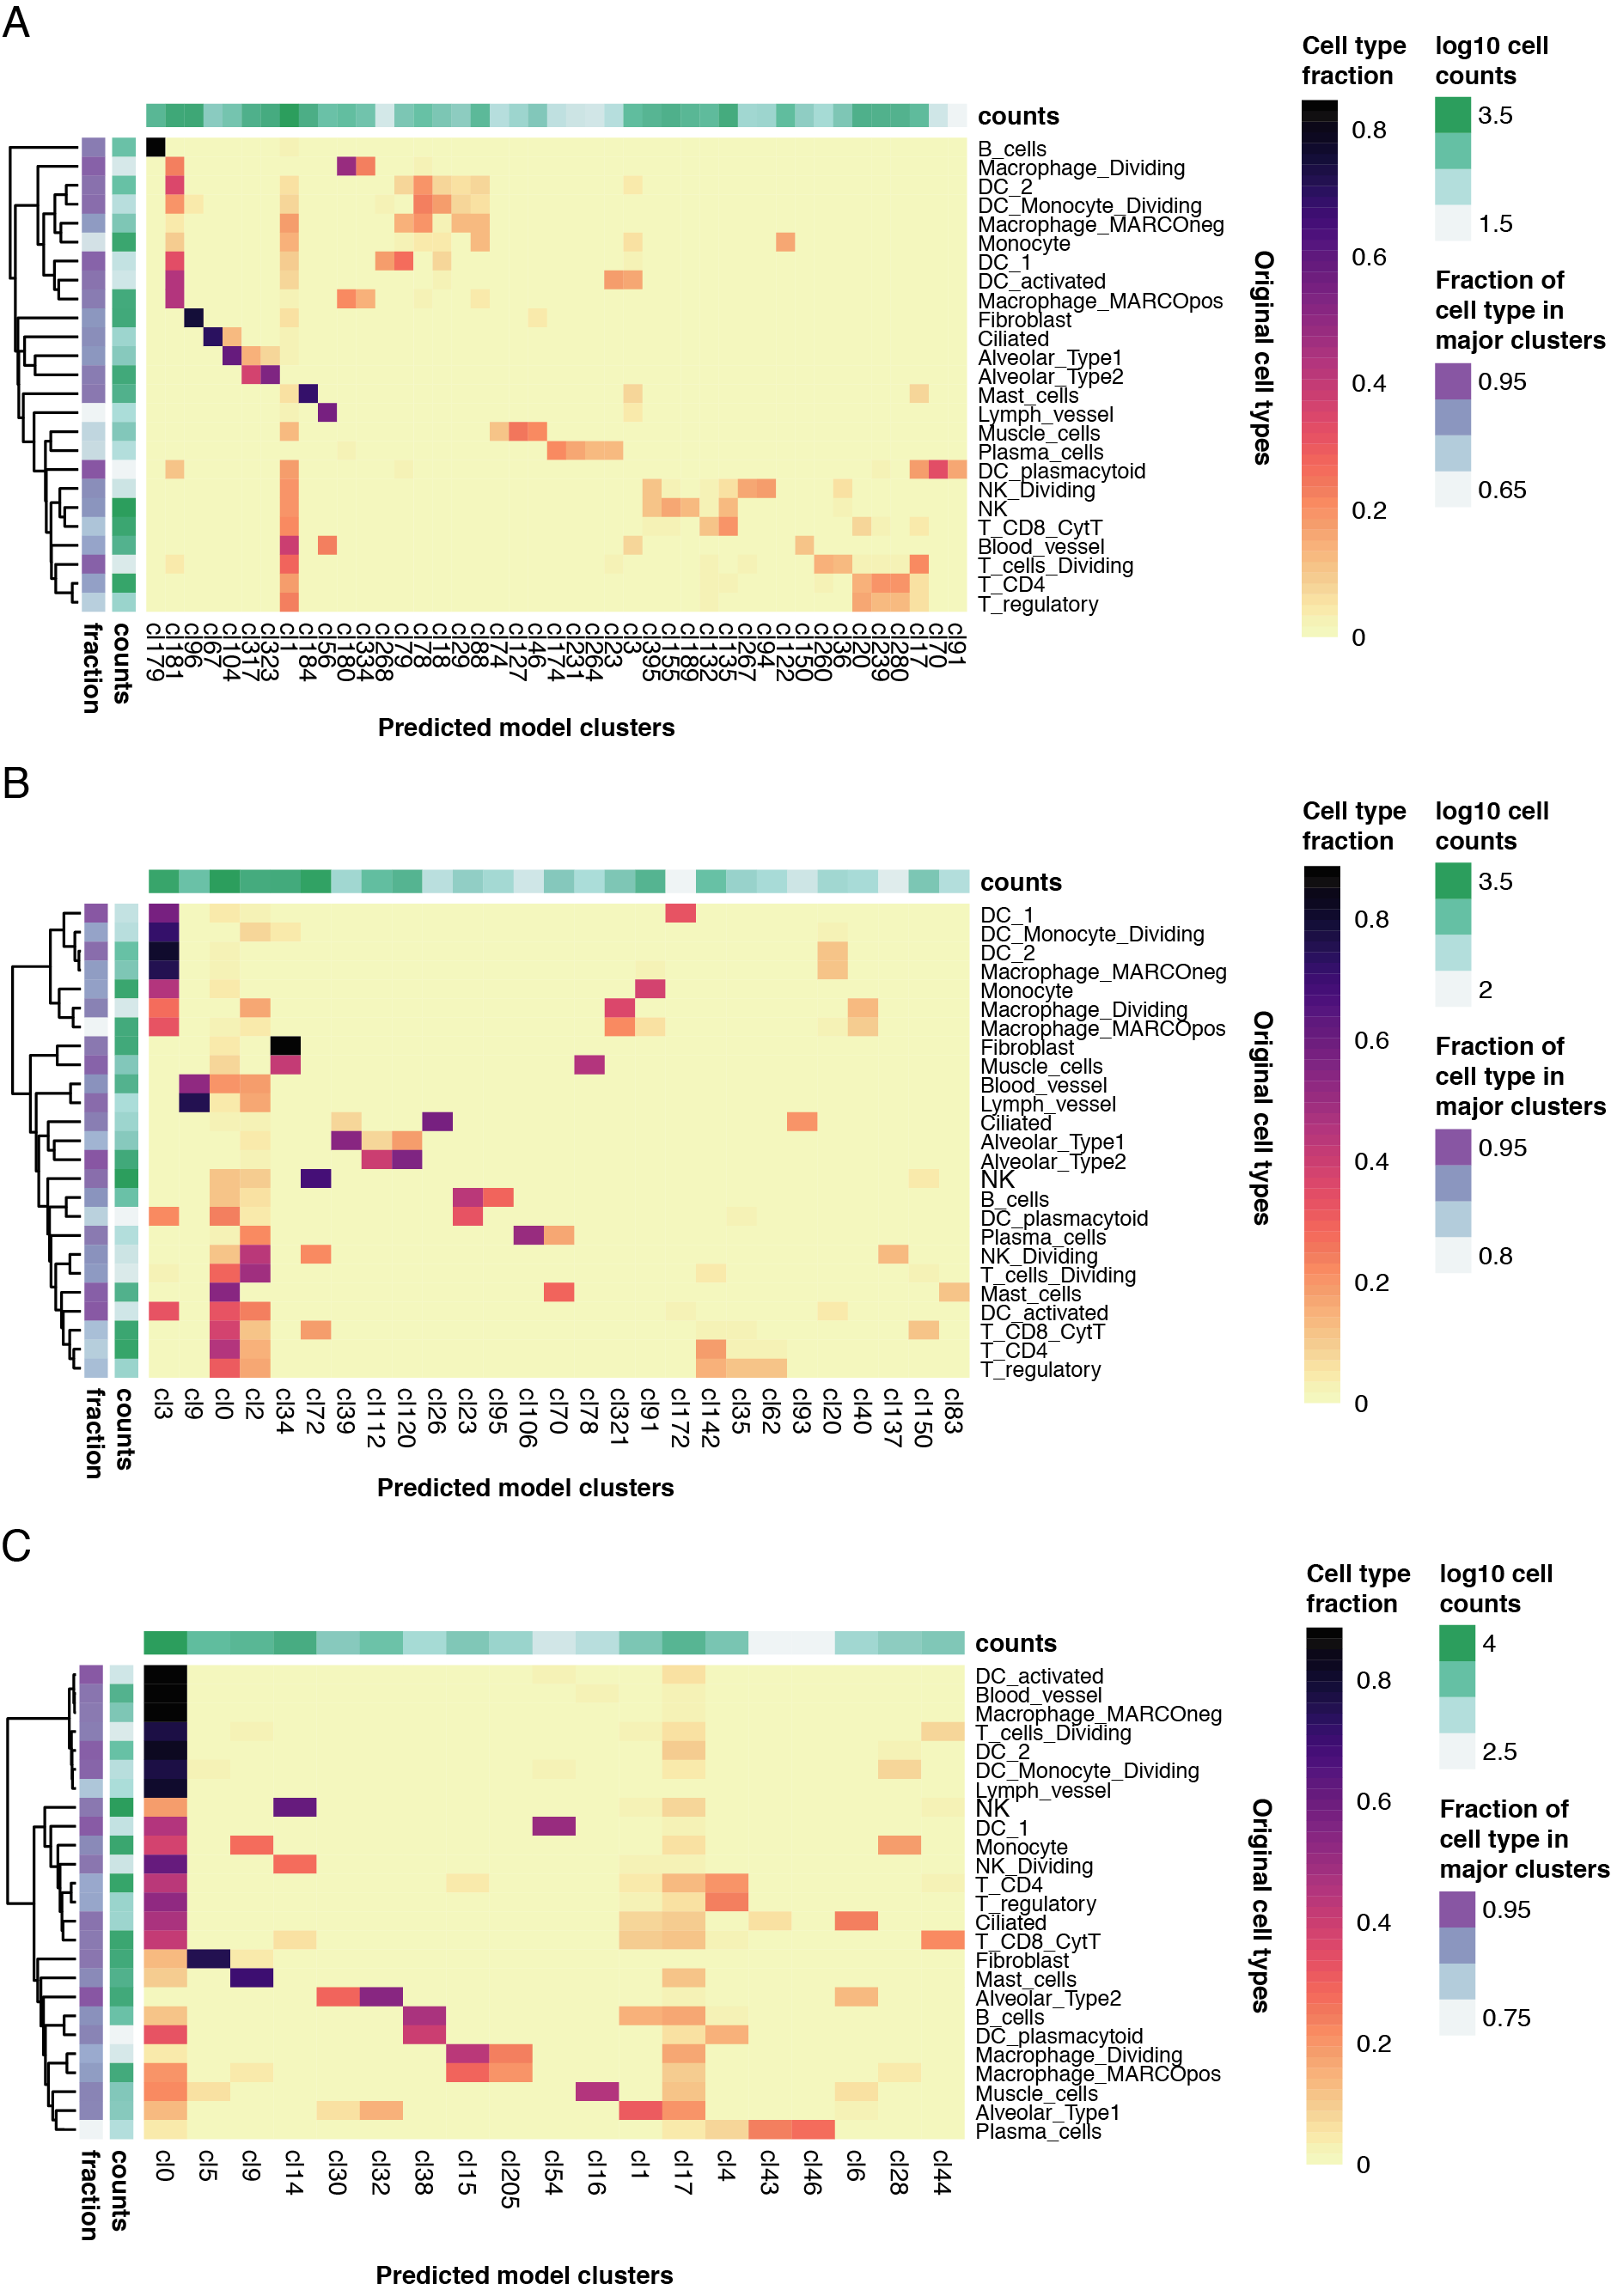
\includegraphics[scale=0.83]{Appendix2/Figs/appB_otherCtFrac_lung.png} % change word in curlies to change figure
\caption[Lung annotated cell types matching clusters in other \textit{CellTypist} models]{\textbf{Lung annotated cell types matching clusters in other \textit{CellTypist} models (Related to Figure~\ref{fig:chap4_preds}C)}\newline Proportion of annotated cell types (rows) included in each cluster (columns) in the models thr1 = 0.4, thr2 = 0.99 \textbf{(A)}, thr1 = 0.25, thr2 = 0.25 \textbf{(A)}, and thr1 = 0.1, thr2 = 0.1 \textbf{(C)}. Only clusters including at least 10\% of a given cell type were included.}
\label{fig:appB_otherct}
\end{figure}


\section{Supplementary Tables}
\label{sectionB1.2}

\begin{table}[ht!] % p for putting it in the next page available
\footnotesize
\caption[Top genes in the largest merged clusters of each \textit{CellTypist} model]{Top genes in the largest merged clusters of each \textit{CellTypist} model}
\centering
\label{table:tab_appB_clgenes}

\begin{tabular}{l|l|l}
\toprule
~\textbf{Model} & ~\textbf{Cluster} & ~\textbf{Top Genes} \\
\midrule
thr1 = 0.99, thr2 = 0.8 & cl87 & \specialcell[t]{S100A4, FOS, KLRB1, DUSP1, NFKBIA, KLF6,\\LTB, CXCR4, ANXA1, SRGN} \\
 & cl147 & \specialcell[t]{HBG2, EEF1A1, RNASE1, HMOX1, RPL39,AL138963.3,\\AC026803.1, H3F3A, EGFL7, FP671120.4}  \\
 & cl102 & \specialcell[t]{C7, DCN, DLK1, IGF2, COL3A1, COL1A1,\\HSPA1A, TSHZ2, HSPA1B, MMP2} \\
 & cl155 & \specialcell[t]{IGLL1, VPREB1, HIST1H4C, HMGB2, H3F3A, PTTG1,\\IL7R, CD24, SMC4, HMGA1} \\
 & cl160 & \specialcell[t]{MT-RNR2, MT-TT, MT-TG, SNORA31, MT-RNR1,\\MTCO1P40, MT-TK, EEF1A1P5, MT2A, Y\_RNA} \\
 
\midrule
thr1 = 0.4, thr2 = 0.99 & cl263 & \specialcell[t]{RPL10P9, RPS3A, DONSON, RPL9, RPS10, AL031280.1,\\SELENOM, RPS26, DPY30, RPL7}  \\
 & cl530 & \specialcell[t]{PPBP, MT-RNR1, GNG11, HIST1H2AC, MIR1244-2,\\NCOA4, GPX1, PF4, OAZ1, CAVIN2}  \\
 & cl215 & \specialcell[t]{GLRX, REXO2, CPVL, GYPB, HIST1H4C, FAM178B,\\HEMGN, RGS16, TUBA3C, GIHCG}  \\
 & cl234 & \specialcell[t]{GNLY, CD52, NKG7, GZMH, CD3D, CD3G,\\IL32, TRGC2, TRAC, TRBC1}  \\
 & cl233 & \specialcell[t]{IGLC2, IGLC3, HLA-DRA, CD74, AL365357.1, CD52,\\ MIR1244-2, MTATP6P1, HLA-DQB1, AC005912.1}  \\
 
\midrule
thr1 = 0.25, thr2 = 0.25 & cl114 & \specialcell[t]{FN1, TPT1, MARCO, RPL10, SARAF, EEF1A1,\\PS3A, TIMP3, RPS29, AL365357.1}  \\
 & cl72 & \specialcell[t]{CCL3L1, AL450405.1, RPL41, KLRF1, IGHA1, DUSP4,\\GZMK, CCL4L1, TYROBP, CCN1}  \\
 & cl102 & \specialcell[t]{MTND1P23, RPS26, JUNB, AL450405.1, MTCO1P12,\\RPS4Y1, ACTB, C20orf204, LTB, MIR1244-2}  \\
 & cl10 & \specialcell[t]{PLP1, LINC01116, SELE, HMOX1, IGFBP5, CXCL12,\\MTRNR2L8, TFPI2, HBG1, APOE}  \\
 & cl23 & \specialcell[t]{ AL450405.1, HLA-DRA, AC027290.2, RPL26, CD74,\\RPL39, H3F3A, RPS26, LINC01781, HLA-DRB6}  \\

\midrule
thr1 = 0.1, thr2 = 0.1 & cl10 & \specialcell[t]{AMH, DHRS2, ADAMDEC1, SELE, CRHBP,\\AL450405.1, INS, POSTN, TMEM88, GZMK}  \\
 & cl1 & \specialcell[t]{FAM178B, PNMT, GAL, CCL3L1, SFTPB, GCG,\\RAB38, KLF1, HLA-DRB6, CCL5}  \\
 & cl2 & \specialcell[t]{WFDC1, PHGR1, IGFBP3, PAGE4, BAMBI, MARCO,\\IGSF6, SERPINB3, FRZB, HAPLN1}  \\
 & cl20 & \specialcell[t]{MTND1P23, AL450405.1, NHSL2, ZNF90, JUNB, CPA5,\\MTCO1P12, AL513365.1, RPL9P9, RP11-138A9.2}  \\
 & cl57 & \specialcell[t]{AL365226.1, MTRNR2L12, XAGE2, ANAPC4,\\AC068134.2, IL24, RETREG1, C3, CSF1R, EMX1}  \\

\bottomrule
\end{tabular}
\end{table}
